\documentclass[aspectratio=169]{beamer}	
\mode<presentation>
 
\usepackage{pdfpages}
\usepackage{fancyvrb}
\usepackage{chemarr}

\usepackage{amsmath}		%% mathematics typesetting
\usepackage{amssymb}
 
\usepackage{epigraph}   %% nice setting of quotations

\usepackage{tabularx} %% allows to use row colours in tables

\usepackage{ulem}

\usepackage{booktabs}

\usepackage{siunitx} %% tpyeset SI units

\usepackage{CJKutf8} %% typeset Chinese characters

\usepackage{pdfpages}%% include pdfs

\usepackage{graphicx}
\usepackage{animate} %% show animated gifs

\DeclareMathAlphabet{\mathcalligra}{T1}{calligra}{m}{n}


% Color and Theme. Can be changed. However, this one's quite nice.
\usetheme{Madrid}
\definecolor{theme}{rgb}{0.84,0,0.21}
\usecolortheme[named=theme]{structure}

%%  Title information
\title[M11.13.1 Psychophysik]{M11.13.1 Psychophysik: \\ Allgemeine Sinneswahrnehmung}
\author[melanie.stefan@medicalschool-berlin.de]{}
\institute[]{Prof. Melanie Stefan \\ melanie.stefan@medcialschool-berlin.de}
\date{Letzte Änderung: SoSe 2025}
 

% Table of contents to pop up at the beginning of each section
\AtBeginSection[]
{
  \begin{frame}<beamer>
    \frametitle{Outline}
    \tableofcontents[currentsection,currentsubsection]
  \end{frame}
}
 
\beamertemplatenavigationsymbolsempty

\begin{document}


{ \usebackgroundtemplate{
\includegraphics[width=\paperwidth]{MSB_Titelseite_169.pdf}} 
\begin{frame}

 \maketitle 

$\,$\\[6cm] 


\end{frame} 
}


\includepdf[pages=-]{progress_test.pdf}

%% Hook:

{ \usebackgroundtemplate{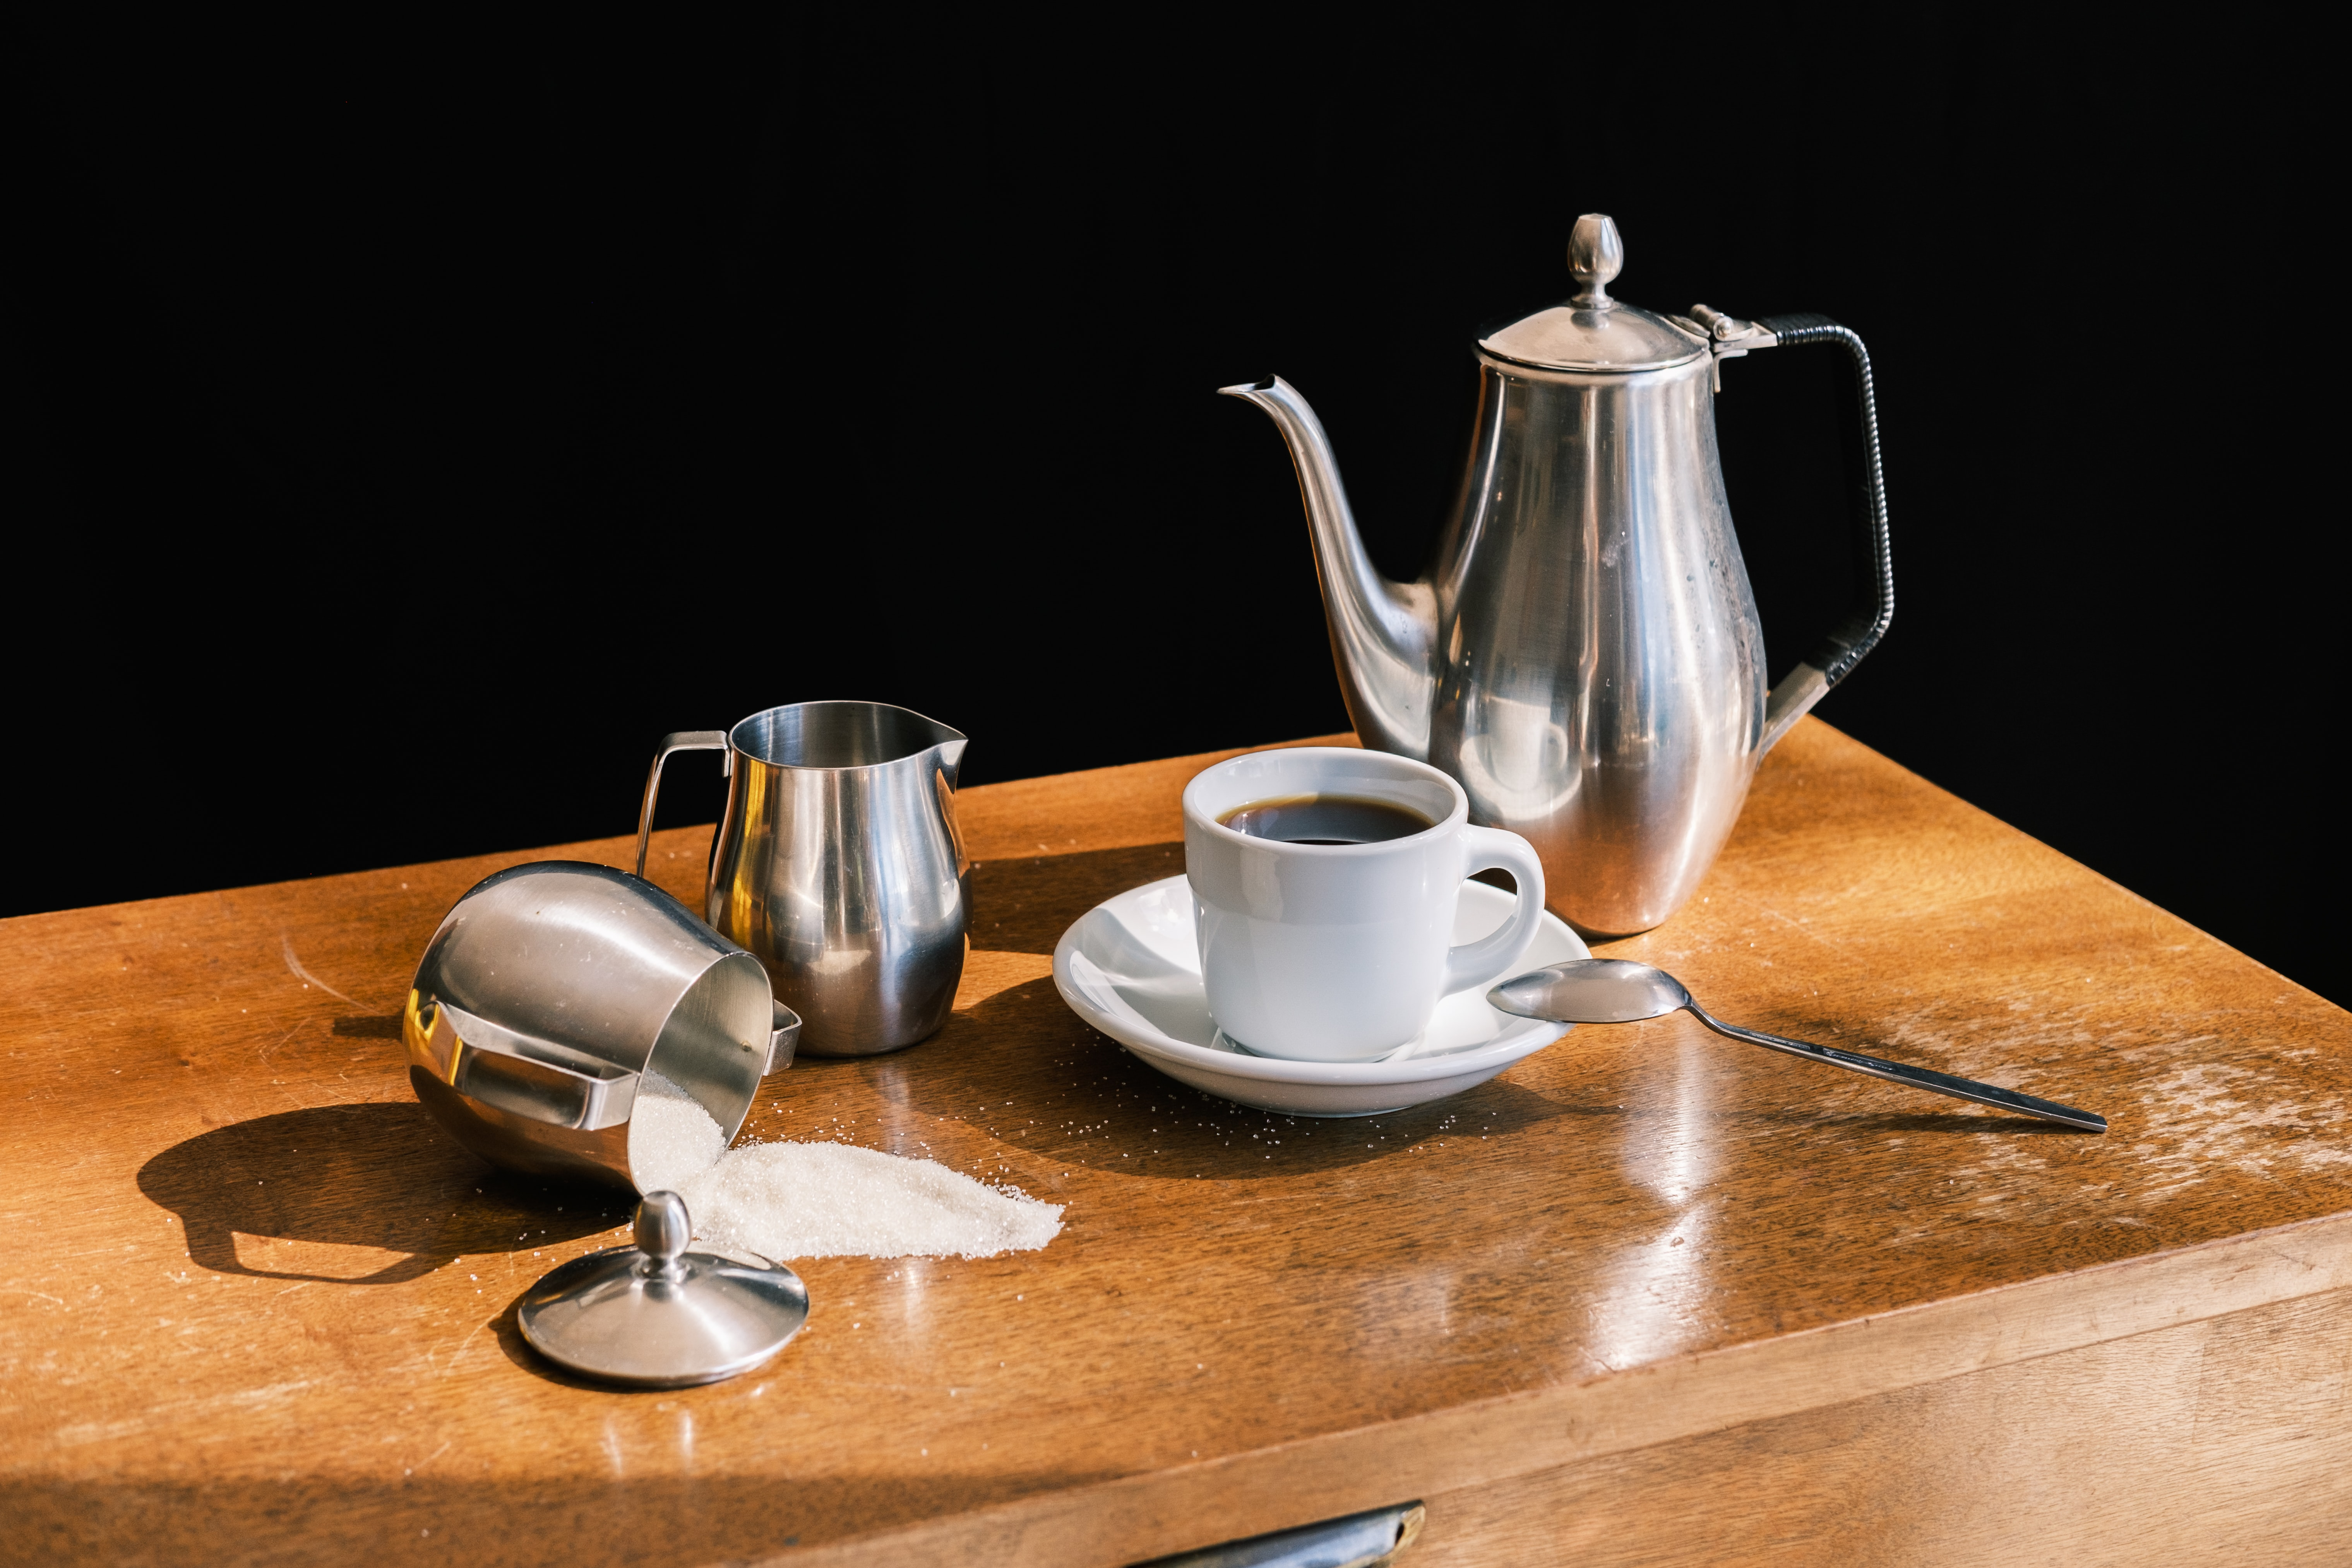
\includegraphics[width=1\paperwidth]{still_life.jpg}} 
\begin{frame}
\textcolor{white}{Wir nehmen die Welt durch unsere Sinne wahr \dots}

$\,$\\[3.5cm]

\pause
\textcolor{white}{Aber wie?}

$\,$\\[4cm]

\end{frame}
}

 
% %% %% TLIA
\begin{frame}{In diesem Semester geht es um Sinnesphysiologie}

Vorlesungen im 4. Semester:

\begin{itemize}
\item
Allgemeine Sinnesphysiologie 
\begin{itemize}
    \item Psychophysik und allgemeine Sinnesphysiologie
\end{itemize}
\item
Somatosensorik 
\begin{itemize}
    \item Somatosensorik 1: Tastsinn
    \item Somatosensorik 2: Propriozeption und Thermorezeption
    \item Somatosensorik 3: Nozizeption und Schmerz
\end{itemize} 
\item Visuelles System 
    \begin{itemize}
    \item
    Visuelles System 1: Dioptrischer Apparat 
    \item
    Visuelles System 2: Retinale Signalverarbeitung, zentrale Sehbahn 
    \end{itemize}
\item
Gehör und Gleichgewicht 
\begin{itemize}
    \item Auditorisches System: Hören und periphere Hörbahnen 
    \item Vestibuläres System
    
\end{itemize}
\item     Chemische Sinne
\begin{itemize}
    \item 
    Chemosensorik: Geschmack und Geruch
\end{itemize}
    
\end{itemize}


(Der Rest sind Repetitorien)

\end{frame}

\begin{frame}{Vorbereitung auf die mündliche M1}

\begin{columns}[c]
    \begin{column}{5cm}
\begin{enumerate}
    \item 
    M1-Tombola in (den meisten) Seminaren
    \item 
    Mündliche Prüfungen in den Repetitorien
\end{enumerate}
        
    \end{column}

    \begin{column}{5cm}
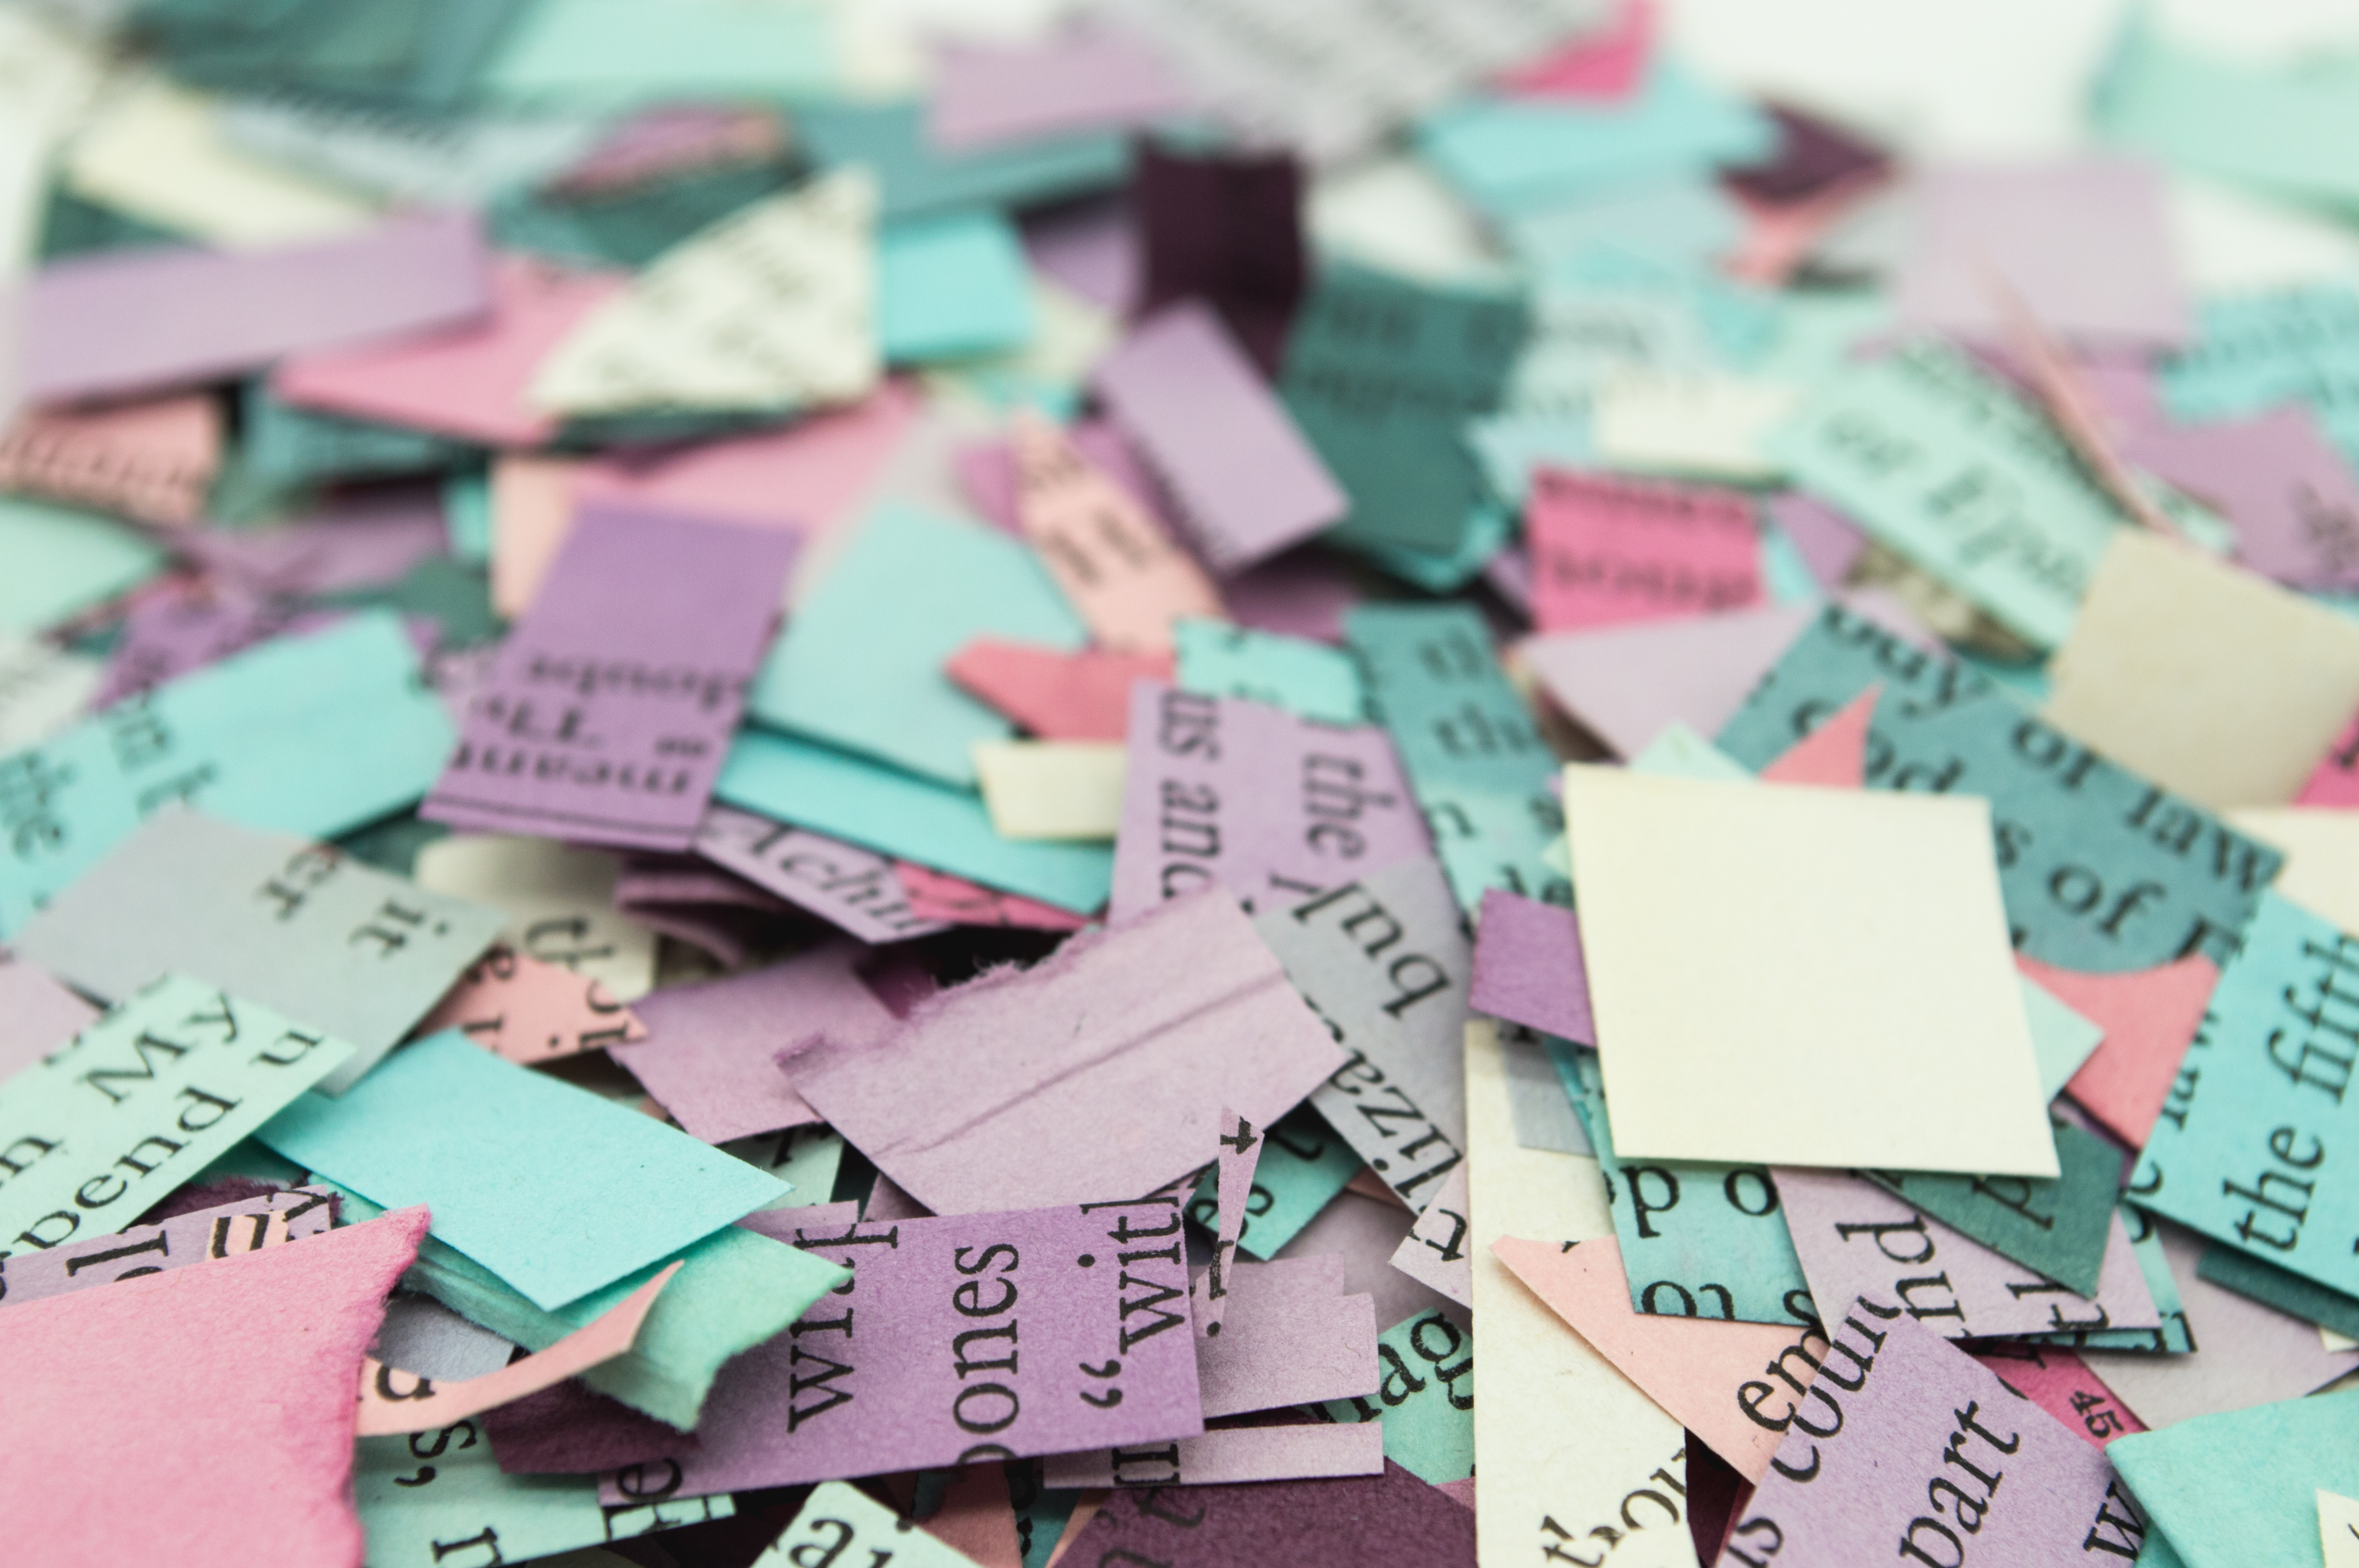
\includegraphics[width=\textwidth]{mel-poole-gT-Sob4njj8-unsplash.jpg}        
    \end{column}

\end{columns}





    
\end{frame}

\begin{frame}{In diesem Semester geht es um Sinnesphysiologie}

Vorlesungen im 4. Semester:

\begin{itemize}
\item
Allgemeine Sinnesphysiologie 
\begin{itemize}
    \item \textcolor{theme}{Psychophysik und allgemeine Sinnesphysiologie}
\end{itemize}
\item
Somatosensorik 
\begin{itemize}
    \item Somatosensorik 1: Tastsinn
    \item Somatosensorik 2: Propriozeption und Thermorezeption
    \item Somatosensorik 3: Nozizeption und Schmerz
\end{itemize} 
\item Visuelles System 
    \begin{itemize}
    \item
    Visuelles System 1: Dioptrischer Apparat 
    \item
    Visuelles System 2: Retinale Signalverarbeitung, zentrale Sehbahn 
    \end{itemize}
\item
Gehör und Gleichgewicht 
\begin{itemize}
    \item Auditorisches System: Hören und periphere Hörbahnen 
    \item Vestibuläres System
    
\end{itemize}
\item     Chemische Sinne
\begin{itemize}
    \item 
    Chemosensorik: Geschmack und Geruch
\end{itemize}
    
\end{itemize}


(Der Rest sind Repetitorien)

\end{frame}



%  % Learning Objectives
 
\begin{frame}

 \frametitle{Nach dieser Vorlesung sollten Sie folgendes können}



\begin{block}{Grundlagen:}




\begin{itemize}

    \item 
Die Begriffe Modalität, Qualität und Intensität erklären
    \item 
Erklären, was eine Schwellenbestimmung ist 
    \item 
Die Gesetze von Weber/Fechner und Stevens anführen und anwenden
    \item 
Adäquate Reize definieren
    \item 
Den allgemeinen Weg der Wahrnehmung vom Reiz zu den entsprechenden Zentren im Gehirn erläutern 
    \item 
Effekte von neuronalen Netzwerken auf die Reizwahrnehmung erklären
\end{itemize}


\end{block}



 

\begin{block}{Klinik:}

\begin{itemize}
    
\item 
Methoden zur Bestimmung von Schwellen erläutern 
\item
Agnosie erklären und ein Beispiel geben
\item
Synästhesie erklären und ein Beispiel geben


\end{itemize}


\end{block}



\end{frame}



%% %% %% Main Body
 

\section{Was nehmen wir wahr?}


%% Modalität, Intensität, Qualtiät
\begin{frame}{Wichtige Begriffe}
    
    \begin{columns}[c]
    \begin{column}{5cm}
\includegraphics[width=\textwidth]{doors.jpg}    
    \end{column}
    
    \begin{column}{6cm}
    
    \textbf{Modalität}: Welcher Sinn? (Z.B. Sehen, Hören, Riechen, \dots) \\[0.2 cm]
    
    \textbf{Qualität}: Wie beschaffen? (Z.B. Farbe, Tonhöhe, Geruch, \dots) \\[0.2 cm]
    
    \textbf{Intensität}: Wie stark? \\ (Z.B. Lichtstärke, Lautstärke, Geruchsstärke, \dots) \\[0.2 cm]
    
    \end{column}
    \end{columns}
    
    
\end{frame}


\begin{frame}{Welche Modalitäten gibt es überhaupt?}

Historisch: Die fünf Sinne: 

\begin{center}
    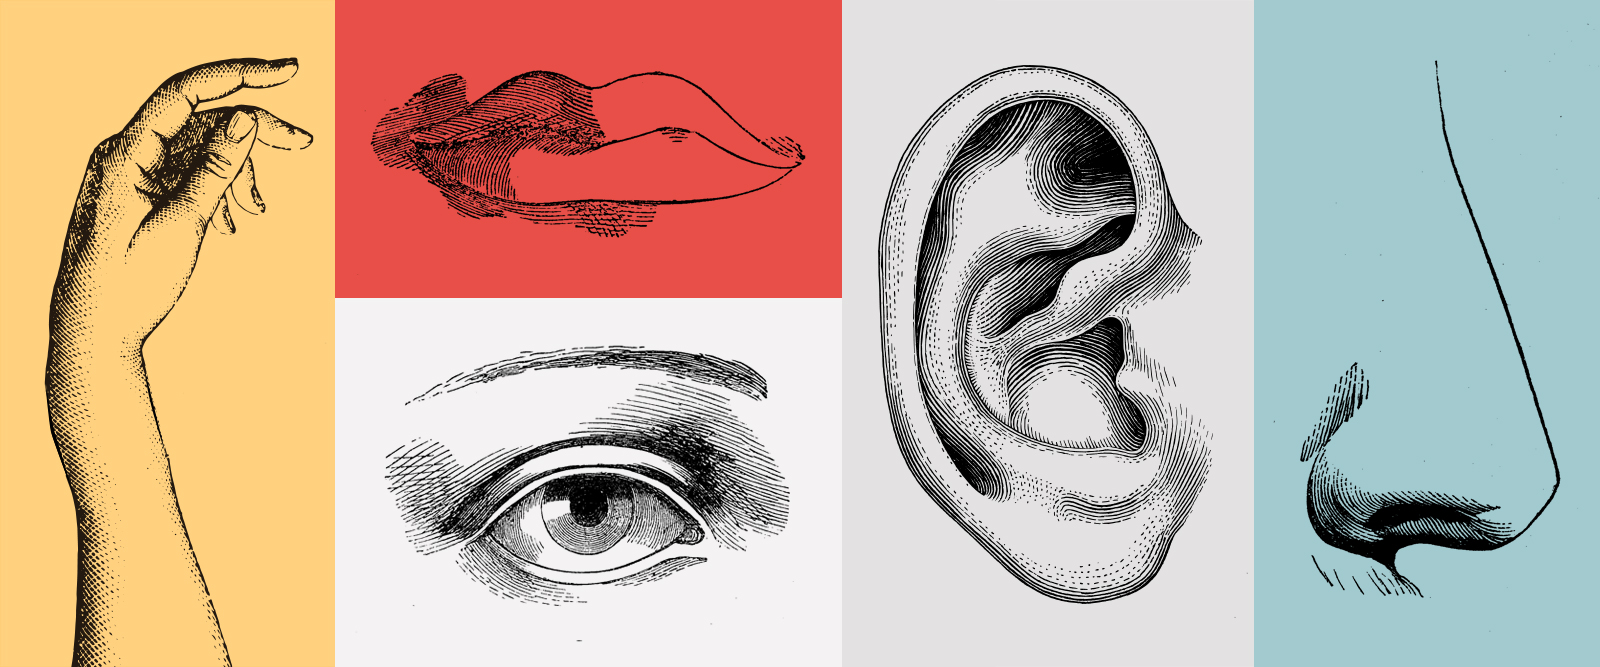
\includegraphics[width=0.9\textwidth]{Five_Senses.jpg}
    
\end{center}

\pause

Welche noch?

\end{frame}



\begin{frame}{Und außerdem: }

Temperatur, Gleichgewicht, Schmerz, Stellung von Gelenken, \dots  \\[0.2 cm]


\pause
Und vielleicht (je nach Definition): Blutdruck, Muskeldehnung, Muskelspannung, Infektion, Hunger, Durst, Harndrang,  \dots 
\end{frame} 



%% Adäquater Reiz oder nicht, Gesetz der spezifischen Sinnesenergien - Synästheie
\begin{frame}{Adäquate und inadäquate Reize}

Sinnesorgane sind auf eine Modalität spezialisiert, können aber manchmal auch durch andere Reizmodalitäten aktiviert werden. \\[0.5 cm]

\pause


Adäquater Reiz: Reiz, für den ein Sensor spezialisiert ist (z.B. Licht für Photorezeptoren im Auge).  \\[0.2 cm]

Inadäquater Reiz: Anderer Reiz, der denselben Sensor trotzdem aktivieren kann (z.B. großer Druck für Photorezeptoren im Auge, "Sterne sehen") \\ [0.2cm]


\end{frame}




\begin{frame}{Gesetz der spezifischen Sinnesenergien}


\begin{block}{Johannes Peter Müller, 1826}

Nicht der äußere Reiz bestimmt die Qualität der Wahrnehmung, sondern nur die Eigenart des gereizten Sinnesorgans.

\end{block}


\pause 
Beispiel? \pause Fühlen von Schallwellen
    
    
\begin{center}
    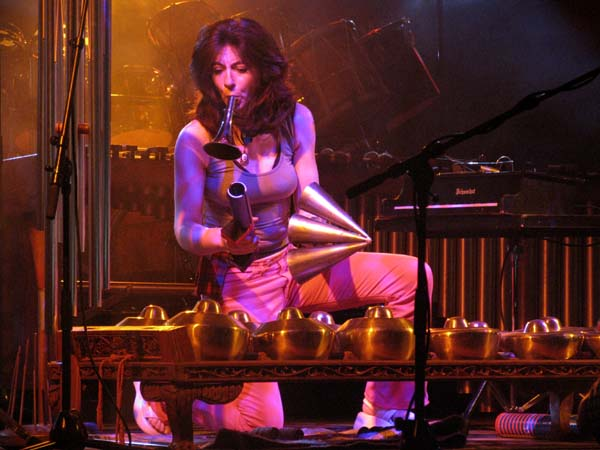
\includegraphics[width=0.4\textwidth]{evelyn_glennie.jpg}
\end{center}


    
\end{frame}




\begin{frame}{Gesetz der spezifischen Sinnesenergien}


\begin{block}{Noch etwas genauer}

Nicht der äußere Reiz bestimmt die Qualität der Wahrnehmung, sondern nur die Eigenart \texbf{der gereizten Wahrnehmungsbahnen}

\end{block}

\begin{columns}[c]

\pause

\begin{column}{7cm}

Beispiel Synästhesie: Reize in einer (Sinnes-)modalität werden (auch) in einer anderen Sinnesmodalität wahrgenommen, z.B. Töne als Farben.

\end{column}

\begin{column}{7cm}
\begin{center}
    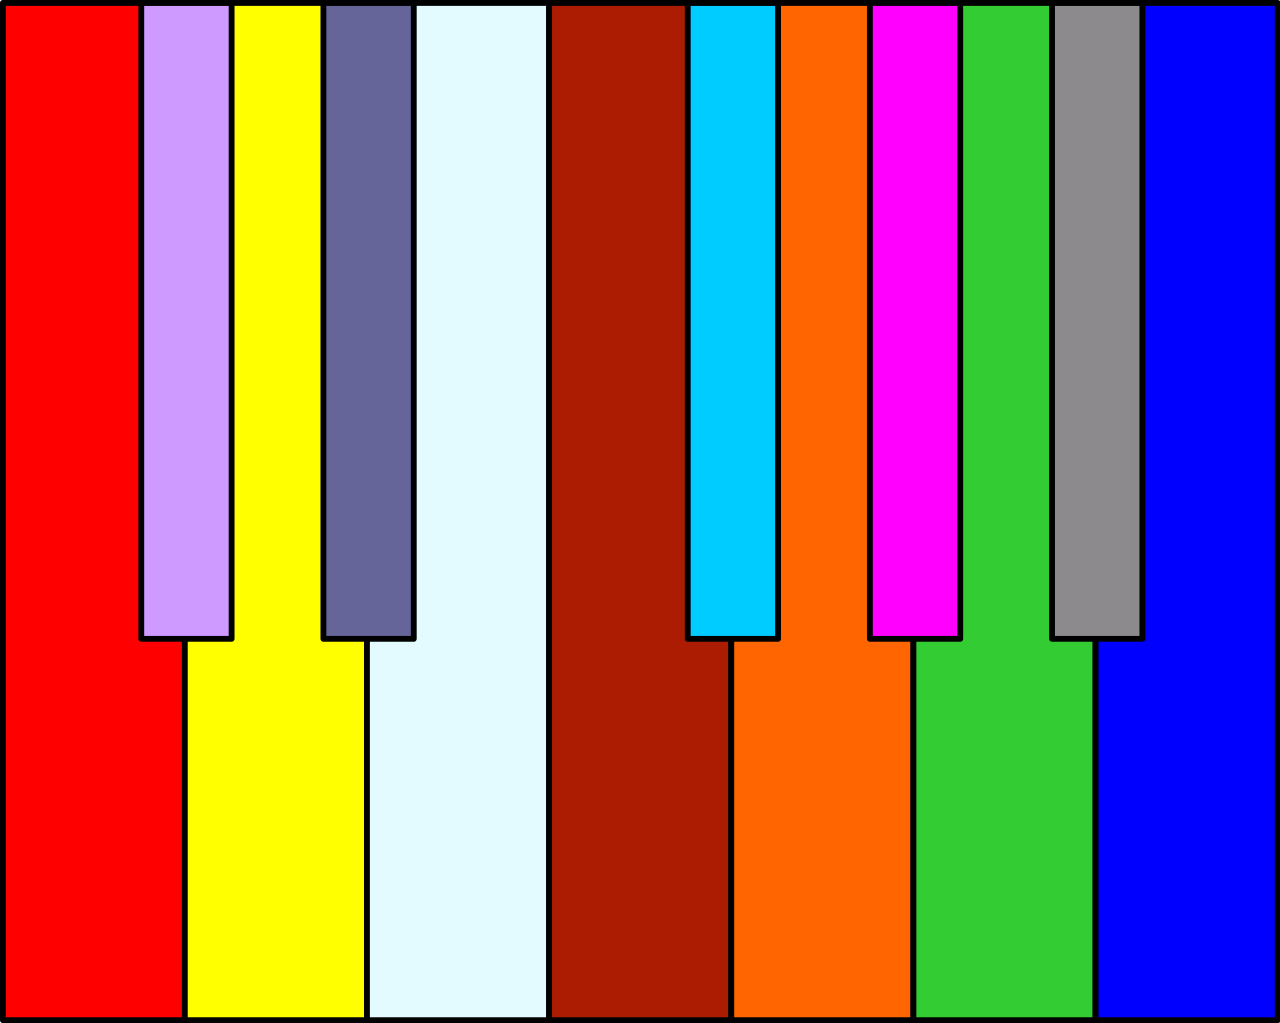
\includegraphics[width=0.8\textwidth]{Scriabin_keyboard.png}
\end{center}

\end{column}




\end{columns}
\end{frame}

\begin{frame}{Beispiel: Zahlen-Farben Synästhesie}
\begin{center}
    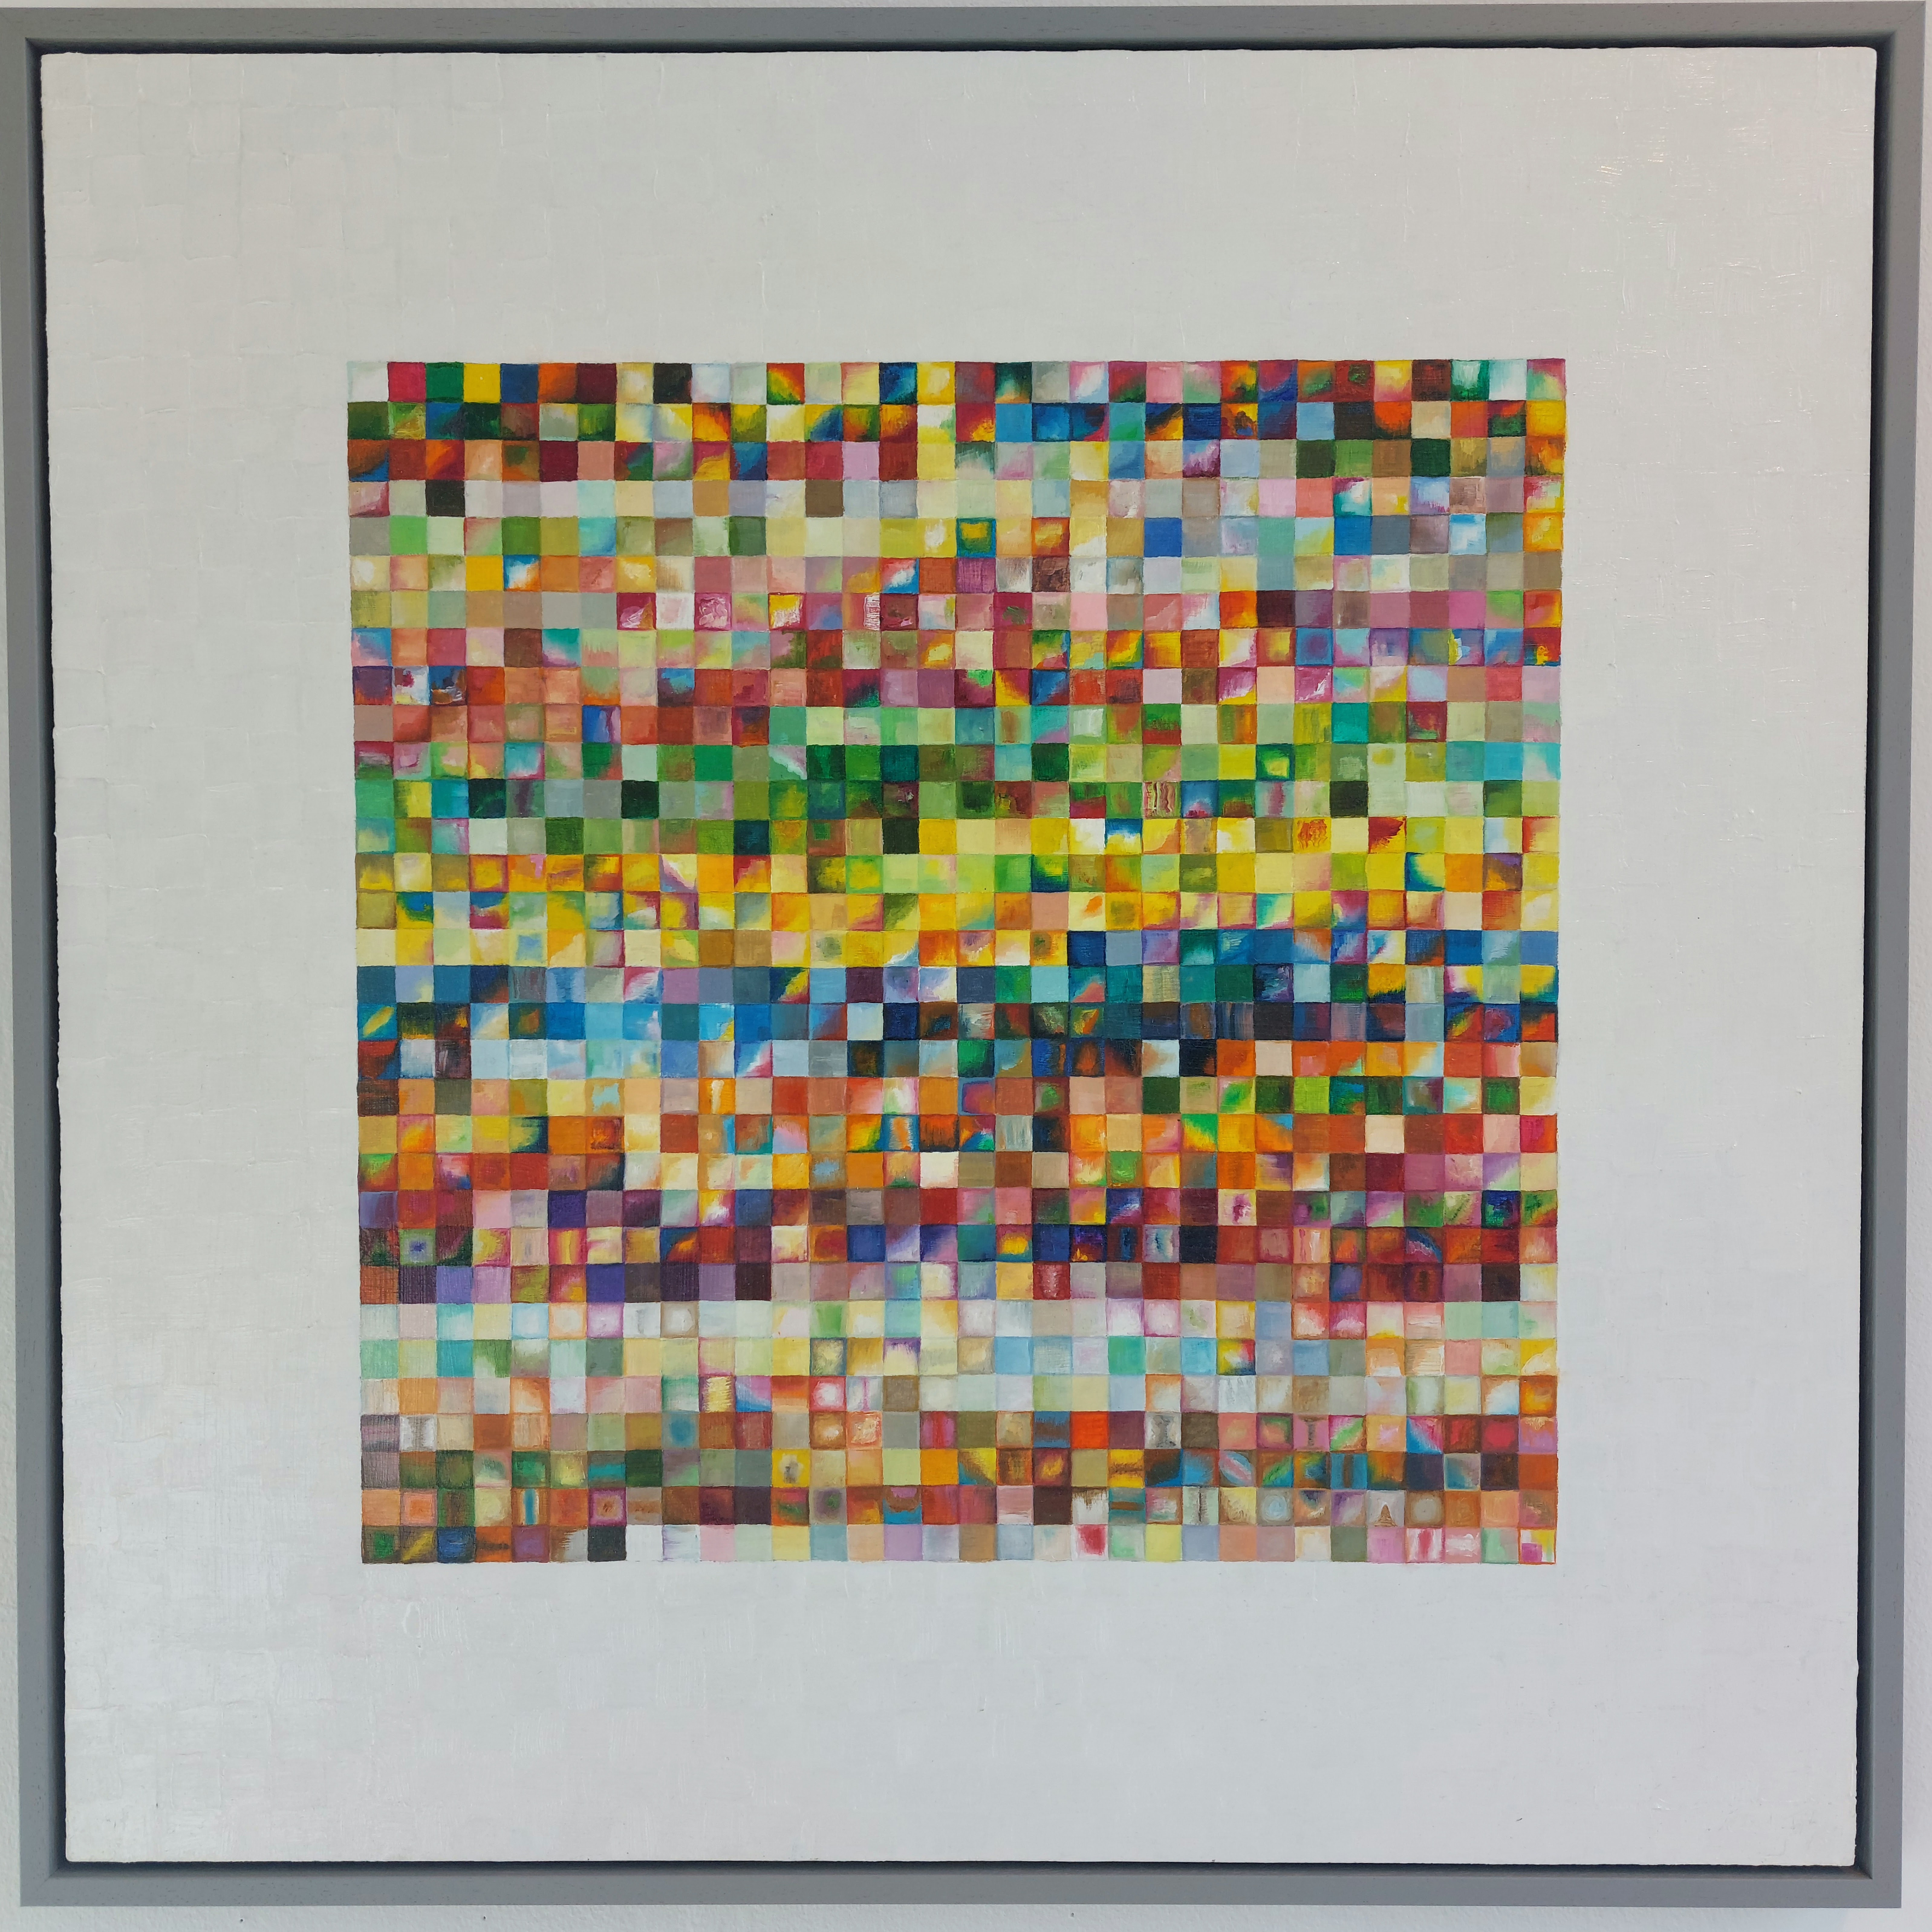
\includegraphics[width=0.4\textwidth]{fliss_inkpen_synesthesia.jpg}
\end{center}


Felicity Inkpen. Synaesthesia: Painting by Numbers (2022) 

\end{frame}

%% cross-modale sinneswahrnehmung

\begin{frame}{Aber: Ein bisschen können wir das alle}

Intermodaler Vergleich: Ausdruck der Qualität und Intensität von Reizen in einer Modalität mit Hilfe einer anderen Modalität ausdrücken.   \\[0.5 cm] \pause 

\begin{block}{Beispiel}
Was ist Bouba, was ist Kiki?
\end{block}
    
    \begin{center}
        
\includegraphics[width=0.6\textwidth]{Booba-Kiki.png}
    \end{center}
    
    
    
\end{frame}


\begin{frame}{Intermodaler Intensitätsvergleich}


\begin{block}{(Klinisch relevanteres) Beispiel}
Schmerz-Skala: Vergleich der Schmerzintensität mit Zahl oder Position entlang der x-Achse (manchmal auch: Farbe)

\end{block}

$\,$\\[0.5 cm]

\begin{center}
    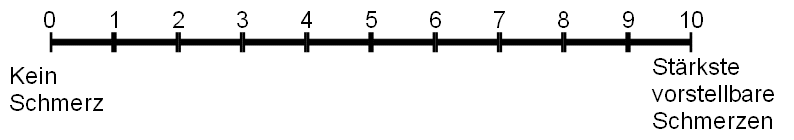
\includegraphics[width=\textwidth]{Numerische_Rating-Skala.png}
\end{center}



\end{frame}


\section{Wie nehmen wir es wahr?}


\begin{frame}{Naive Sicht}

\begin{center}
    \includegraphics[width=0.8\textwidth]{perception_naive.png}
\end{center}
    
\end{frame}


\begin{frame}{Aber in Wirklichkeit \dots}

Im Wahrnehmungsprozess werden Reize umgewandelt, gefiltert, verstärkt, etc.  Eindrücke aus verschiedenen Sinnesmodalitäten werden miteinander und mit anderen neuronalen Funktionen (z.B. bereits vorhandenes Wissen, Emotionen, ...) verknüpft.  \\[1cm]

Wahrnehmung dient nicht dazu, ein naturgetreues Abbild der äußeren Welt zu erschaffen, sondern nur dazu, genug Information zu erhalten, um in der Welt zurecht zu kommen. 

\end{frame}


%% Wahrnehmungsbahn allgemein
\begin{frame}{Die Wahrnehmungsbahn}

\begin{center}
    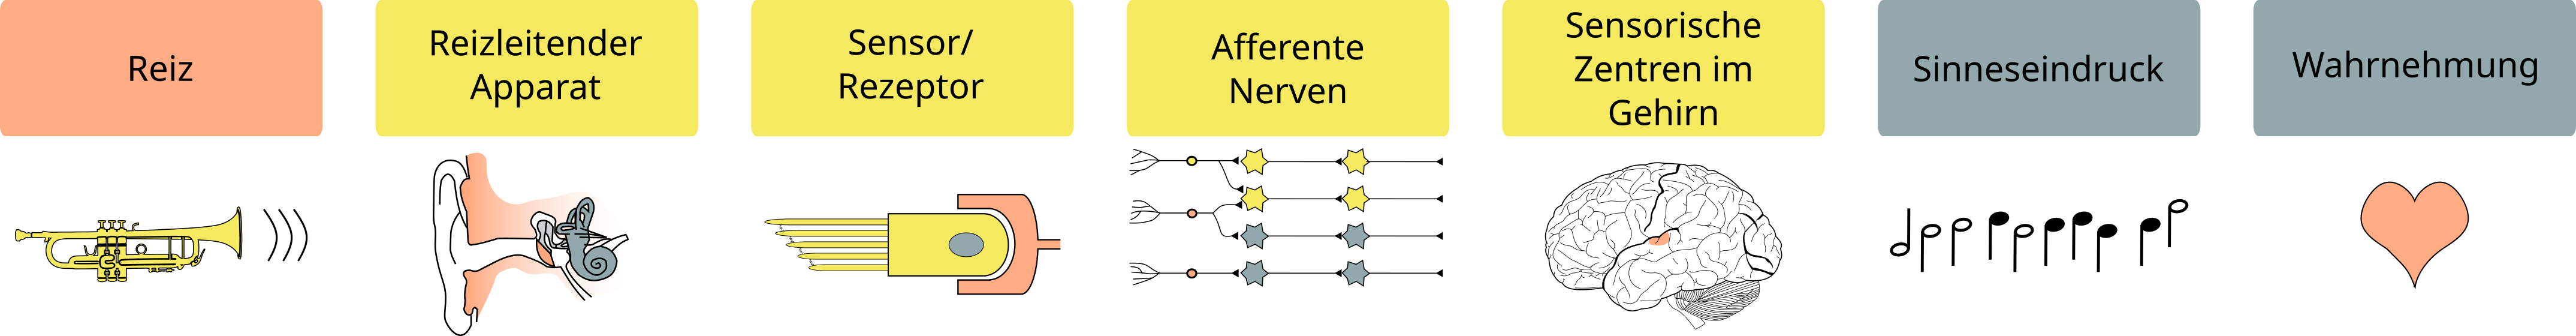
\includegraphics[width=\textwidth]{wahrnehmungsprozess.png}
\end{center}
    
\end{frame}
 
 
 %% Transduktion, Transmission


\begin{frame}{Transduktion und Transmission}

\begin{center}
    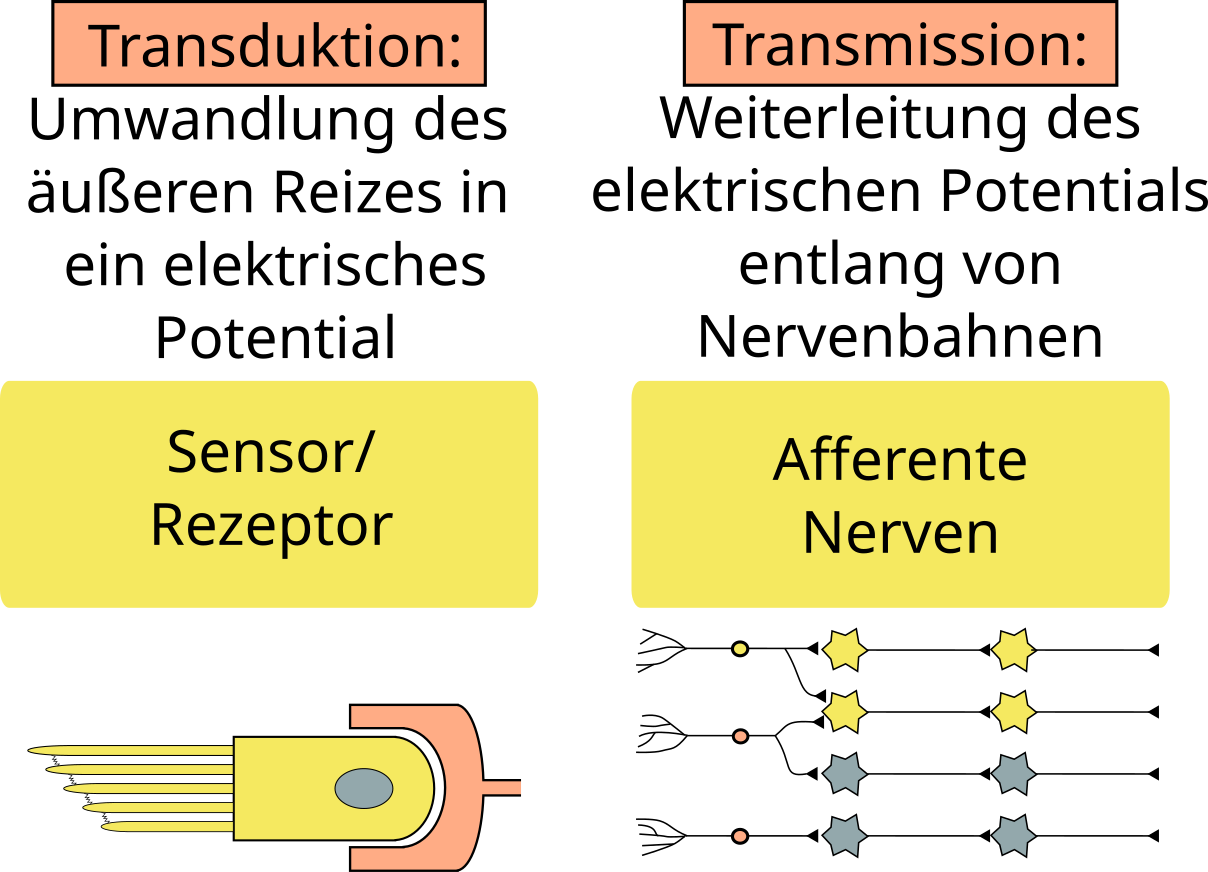
\includegraphics[width=0.6\textwidth]{wahrnehmungsprozess_transduktion_transmission.png}
\end{center}
    
\end{frame}



%% Arten von Rezeptoren, Generatorpotential

%% Sensor Teaserbild

%% Was ist ein Rezeptor?

\begin{frame}{Begriffsklärung: Was ist ein Rezeptor?}

Es ist kompliziert \dots 

Rezeptor kann heißen: 

\begin{itemize}
    \item 
    Eine Sinneszelle (z.B. Photorezeptoren wie Stäbchen und Zapfen beim Sehen) (auch: Sensor)
    \item
    Den Membranbereich einer Sinneszelle, wo Reize in neuronale Information umgewandelt wird (z.B. freie Nervenendigungen, die als Nozizeptoren dienen) (auch: Sensor)
    \item
    Ein Molekül in einer Membran, das Signale auf einer Seite der Membran wahrnimmt Information an die andere Seite weiterleitet (z.B. G-Protein gekoppelte Rezeptoren zur Wahrnehmung von Gerüchen) 
\end{itemize}
    
Die Begrifflichkeit ist nicht eindeutig, daher immer Vorsicht beim Lesen!  

    

\end{frame}






%% Arten von Sinnesrezeptoren

%% Mechano
\begin{frame}{Arten von Sinnesrezeptoren}

\begin{columns}[c]

\begin{column}{7cm}

\begin{block}{Mechanorezeptoren}

Eine mechanische Verformung wird durch Fortsätze an spezialisierten Zellen erfasst und führt (direkt oder indirekt) zu einer Öffnung oder Schließung von Ionenkanälen.  \\

Es entsteht eine Veränderung im Membranpotential.

\pause

Beispiel: Haarzellen in der Cochlea.

\end{block}
\end{column}

\begin{column}{4cm}
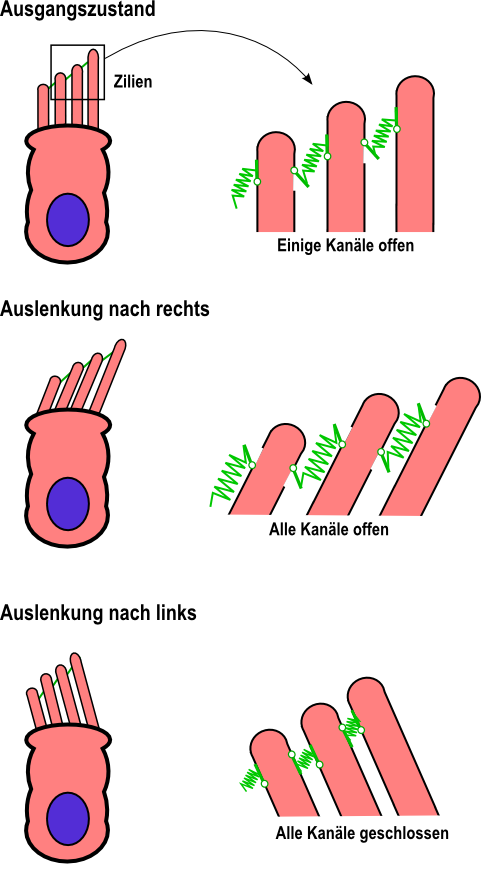
\includegraphics[width=\textwidth]{Haarzelle.png}
\end{column}


\end{columns}


\end{frame} 

%% Chemo
\begin{frame}{Arten von Sinnesrezeptoren}


\begin{block}{Chemorezeptoren}

Bindung eines Moleküls im extrazellulären Teil eines Transmembran-Rezeptors führt zu strukturellen Veränderungen an der Innenseite und dadurch zur Aktivierung von Signalkaskaden. Diese Signalkaskaden führen wieder zur Öffnung von Ionenkanälen, und einer Änderung des Membranpotentials.   \\

Beispiel: Olfaktorische Rezeptoren sind im Prinzip GPCRs vom Typ G\textsubscript{S}. 


\end{block}

\begin{center}
    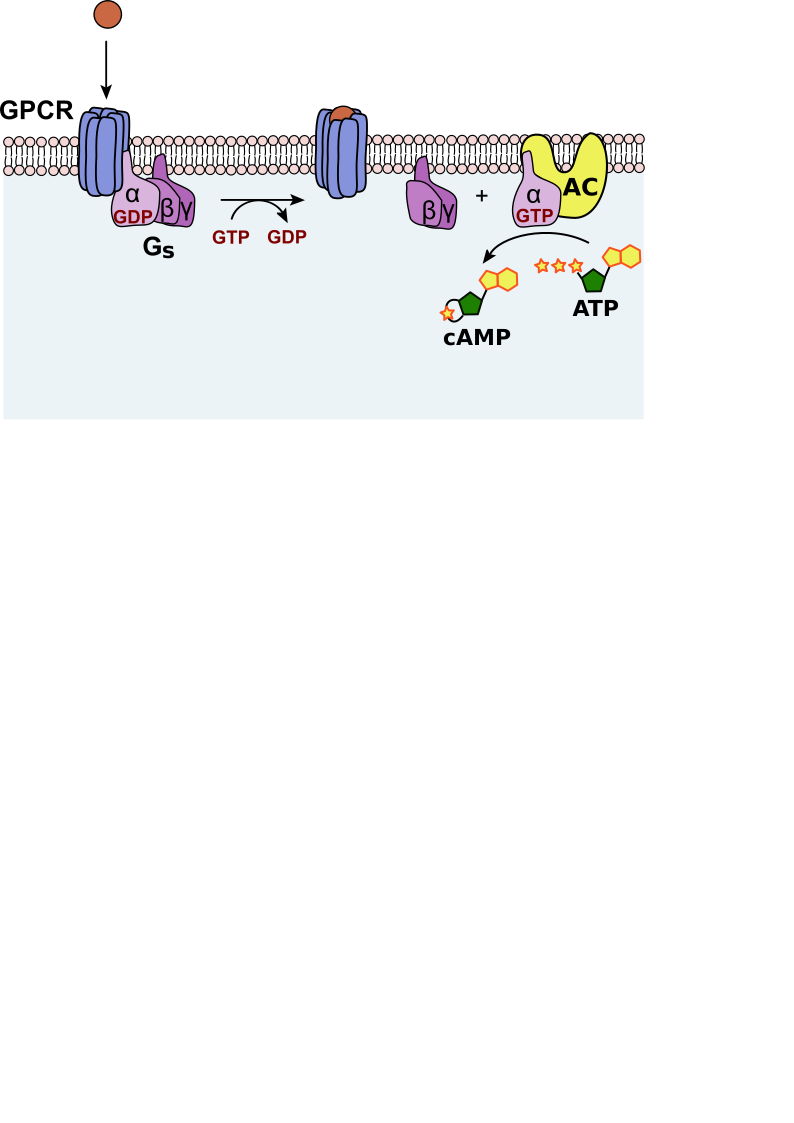
\includegraphics[width=0.6\textwidth]{GPCR_Gs_pathway.png}
\end{center}


\end{frame}


%% Licht
\begin{frame}{Arten von Sinnesrezeptoren}

\begin{columns}[c]

\begin{column}{7cm}

\begin{block}{Energie-Rezeptoren}

Eintreffen von Energie (z.B. Photon, Wärme) an der Außenseite eines Transmembran-Rezeptors bewirkt eine Änderung der Konformation und setzt dadurch Signalkaskaden im Inneren der Zelle in Gang, die zu einer Änderung des Membranpotentials führen. \\

\pause
Beispiel: Rhodopsin in den Stäbchenzellen des Auges ist ein G-Protein gekoppelter Rezeptor.  
\end{block}


\end{column}

\begin{column}{7cm}
\begin{center}

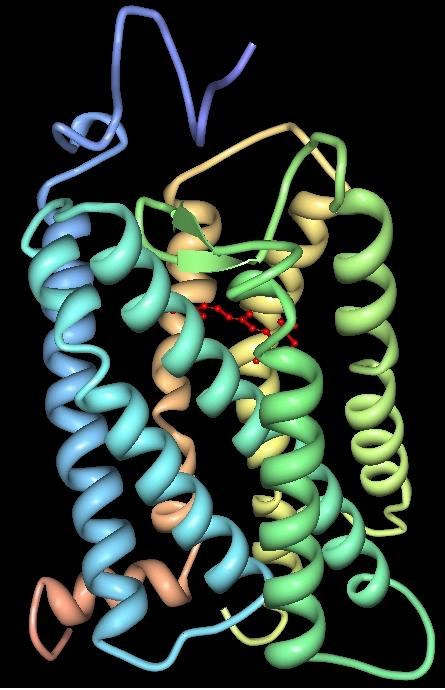
\includegraphics[width=0.6\textwidth]{Rhodopsin_3D.jpg}

\end{center}


\end{column}


\end{columns}

\end{frame}





%% Generatorpotential
\begin{frame}{Generatorpotential}

Die Änderung des Membranpotentials, die durch Aktivierung des Rezeptors hervorgerufen wird, heißt "Generatorpotential" oder "Rezeptorpotential". \\[0.5 cm]

Die Information aus dem Generatorpotential wird in Aktionspotentiale umgewandelt und so weiter übermittelt. (Entweder durch Entstehen von Aktionspotentialen in der selben Zelle, oder durch Freisetzung von Neurotransmittern, die ein Aktionspotential in einer Downstream-Zelle auslösen können.) 


\end{frame}


%% Frequenzkodierung



\begin{frame}{Frequenzcodierung}

\begin{columns}
\begin{column}{7cm}

Die \textbf{Amplitude} des Generatorpotentials wird als \textbf{Frequenz} der Aktionspotentiale codiert. Warum? \\[0.2 cm]
\pause

Weil bei einem größeren Generatorpotential die Schwellenspannung zum Aktionspotential schneller übertreten wird. 
\end{column}

\begin{column}{7cm}
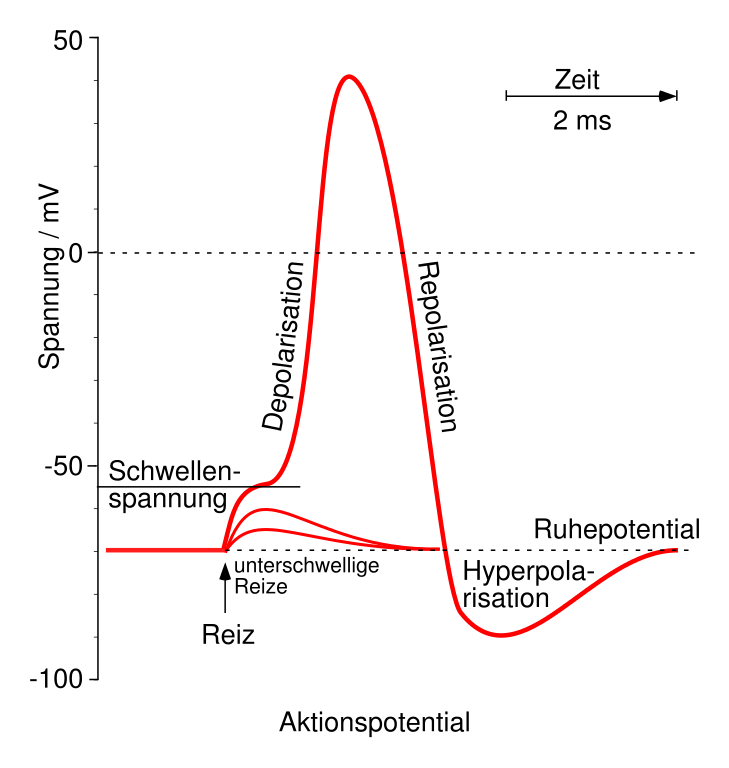
\includegraphics[width=\textwidth]{Aktionspotential.png}
\end{column}

\end{columns}

\end{frame}




% %% Rezeptive Felder
\begin{frame}{Rezeptives Feld}

"Bereich" durch den ein einzelnes Neuron aktiviert werden kann.  \pause

Beispiel: Tastsinn: Räumlicher Bereich

\begin{center}
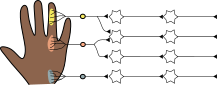
\includegraphics[width=\textwidth]{rezeptives_feld_tasten_primaer.png}    
\end{center}
    
\end{frame}


\begin{frame}{Rezeptives Feld}

"Bereich" durch den ein einzelnes Neuron aktiviert werden kann.  

Beispiel: Chemische Sinne: Ähnlichkeitsbereich \\[0.5 cm]

\begin{center}
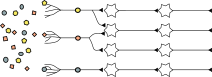
\includegraphics[width=\textwidth]{rezeptives_feld_geruch_primaer.png}    
\end{center}
    
\end{frame}

\begin{frame}{Rezeptives Feld}

Ist ein großes oder kleines rezeptives Feld besser?

\pause

\begin{center}
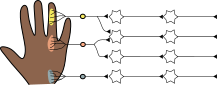
\includegraphics[width=\textwidth]{rezeptives_feld_tasten_primaer.png}    
\end{center}

Kleineres rezeptives Feld bedeutet bessere Unterscheidung von Reizen. 

\end{frame}


\begin{frame}{Sekundäres rezeptives Feld}

\begin{center}
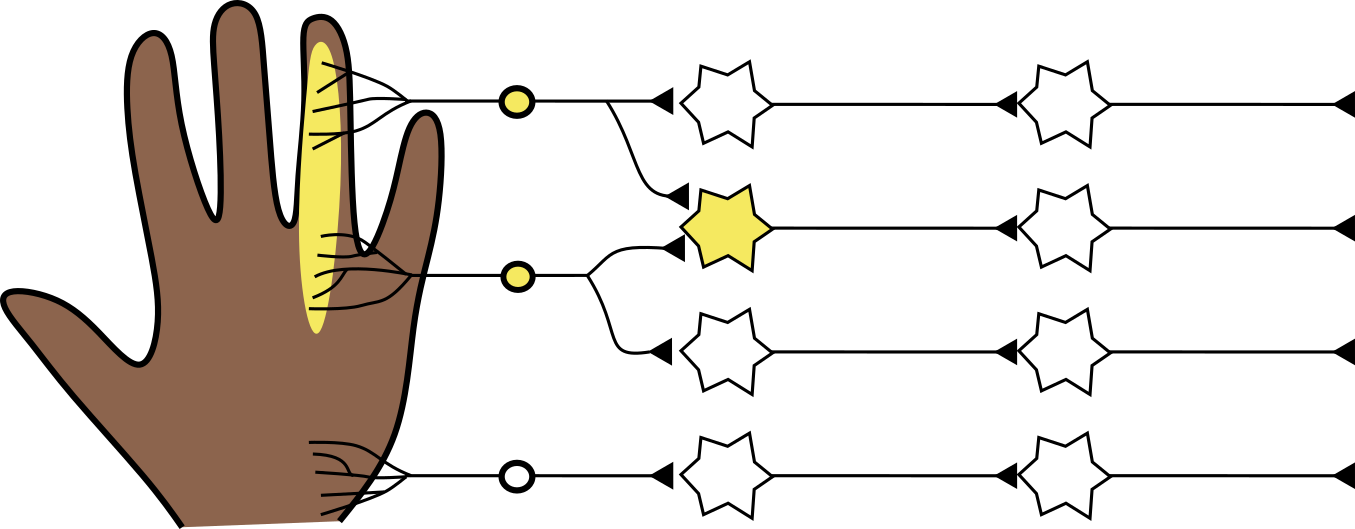
\includegraphics[width=\textwidth]{rezeptives_feld_tasten_sekundaer.png}    
\end{center}


\end{frame}

%% Netzwerk-Effekte: Konvergenz, Divergenz, Laterale Hemmung, Bsp. Kontrastwahrnehmung
\begin{frame}{Netzwerk-Effekte}
\begin{center}
    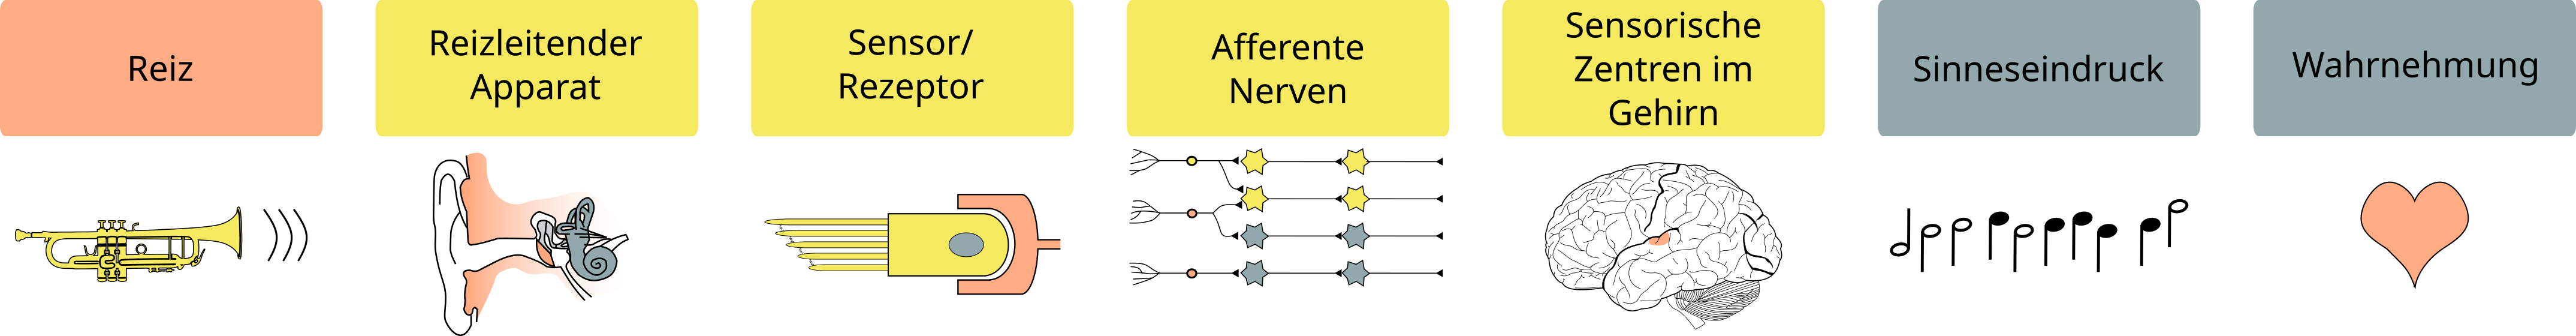
\includegraphics[width=\textwidth]{wahrnehmungsprozess.png}
\end{center}
    
\end{frame}

%% Konvergenz
\begin{frame}{Konvergenz und Divergenz strukturieren die Transmission}

Konvergenz:

\begin{center}
    \includegraphics<1>[width=\textwidth]{konvergenz_1.png}
    \includegraphics<2>[width=\textwidth]{konvergenz_2.png}
\end{center}


\end{frame}



%% Divergenz
\begin{frame}{Konvergenz und Divergenz strukturieren die Transmission}

Divergenz:

\begin{center}
    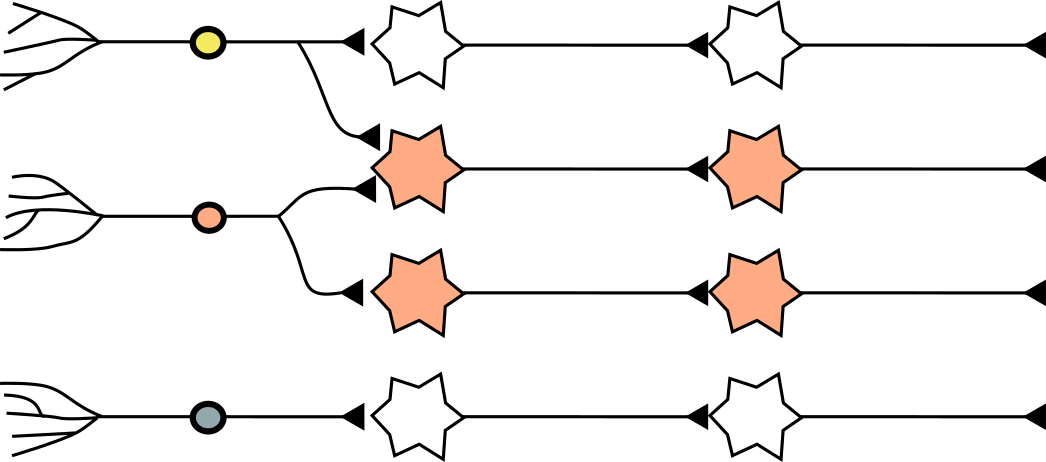
\includegraphics[width=\textwidth]{divergenz.png}
\end{center}


\end{frame}

% Laterale Hemmung

\begin{frame}{Laterale Hemmung}

\begin{center}
    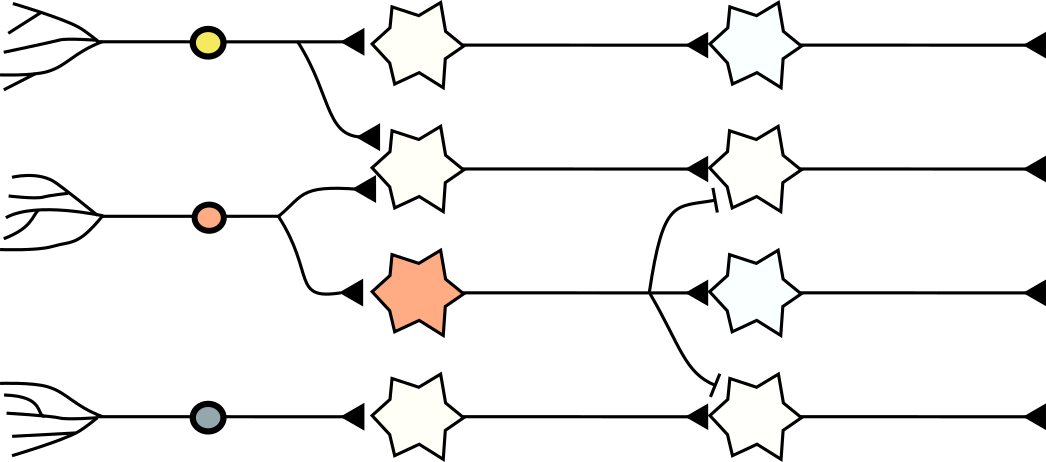
\includegraphics[width=\textwidth]{lateral_inhibition_detail.png}
\end{center}

Wozu?

\end{frame}


\begin{frame}{Laterale Hemmung}

\begin{center}

    \includegraphics<1>[width=\textwidth]{lateral_inhibition_funkction_1.png}
        \includegraphics<2>[width=\textwidth]{lateral_inhibition_funkction_2.png}
\end{center}

\end{frame}


\begin{frame}{Laterale Hemmung dient der Erkennung und Verstärkung von Kontrasten }

\begin{center}
    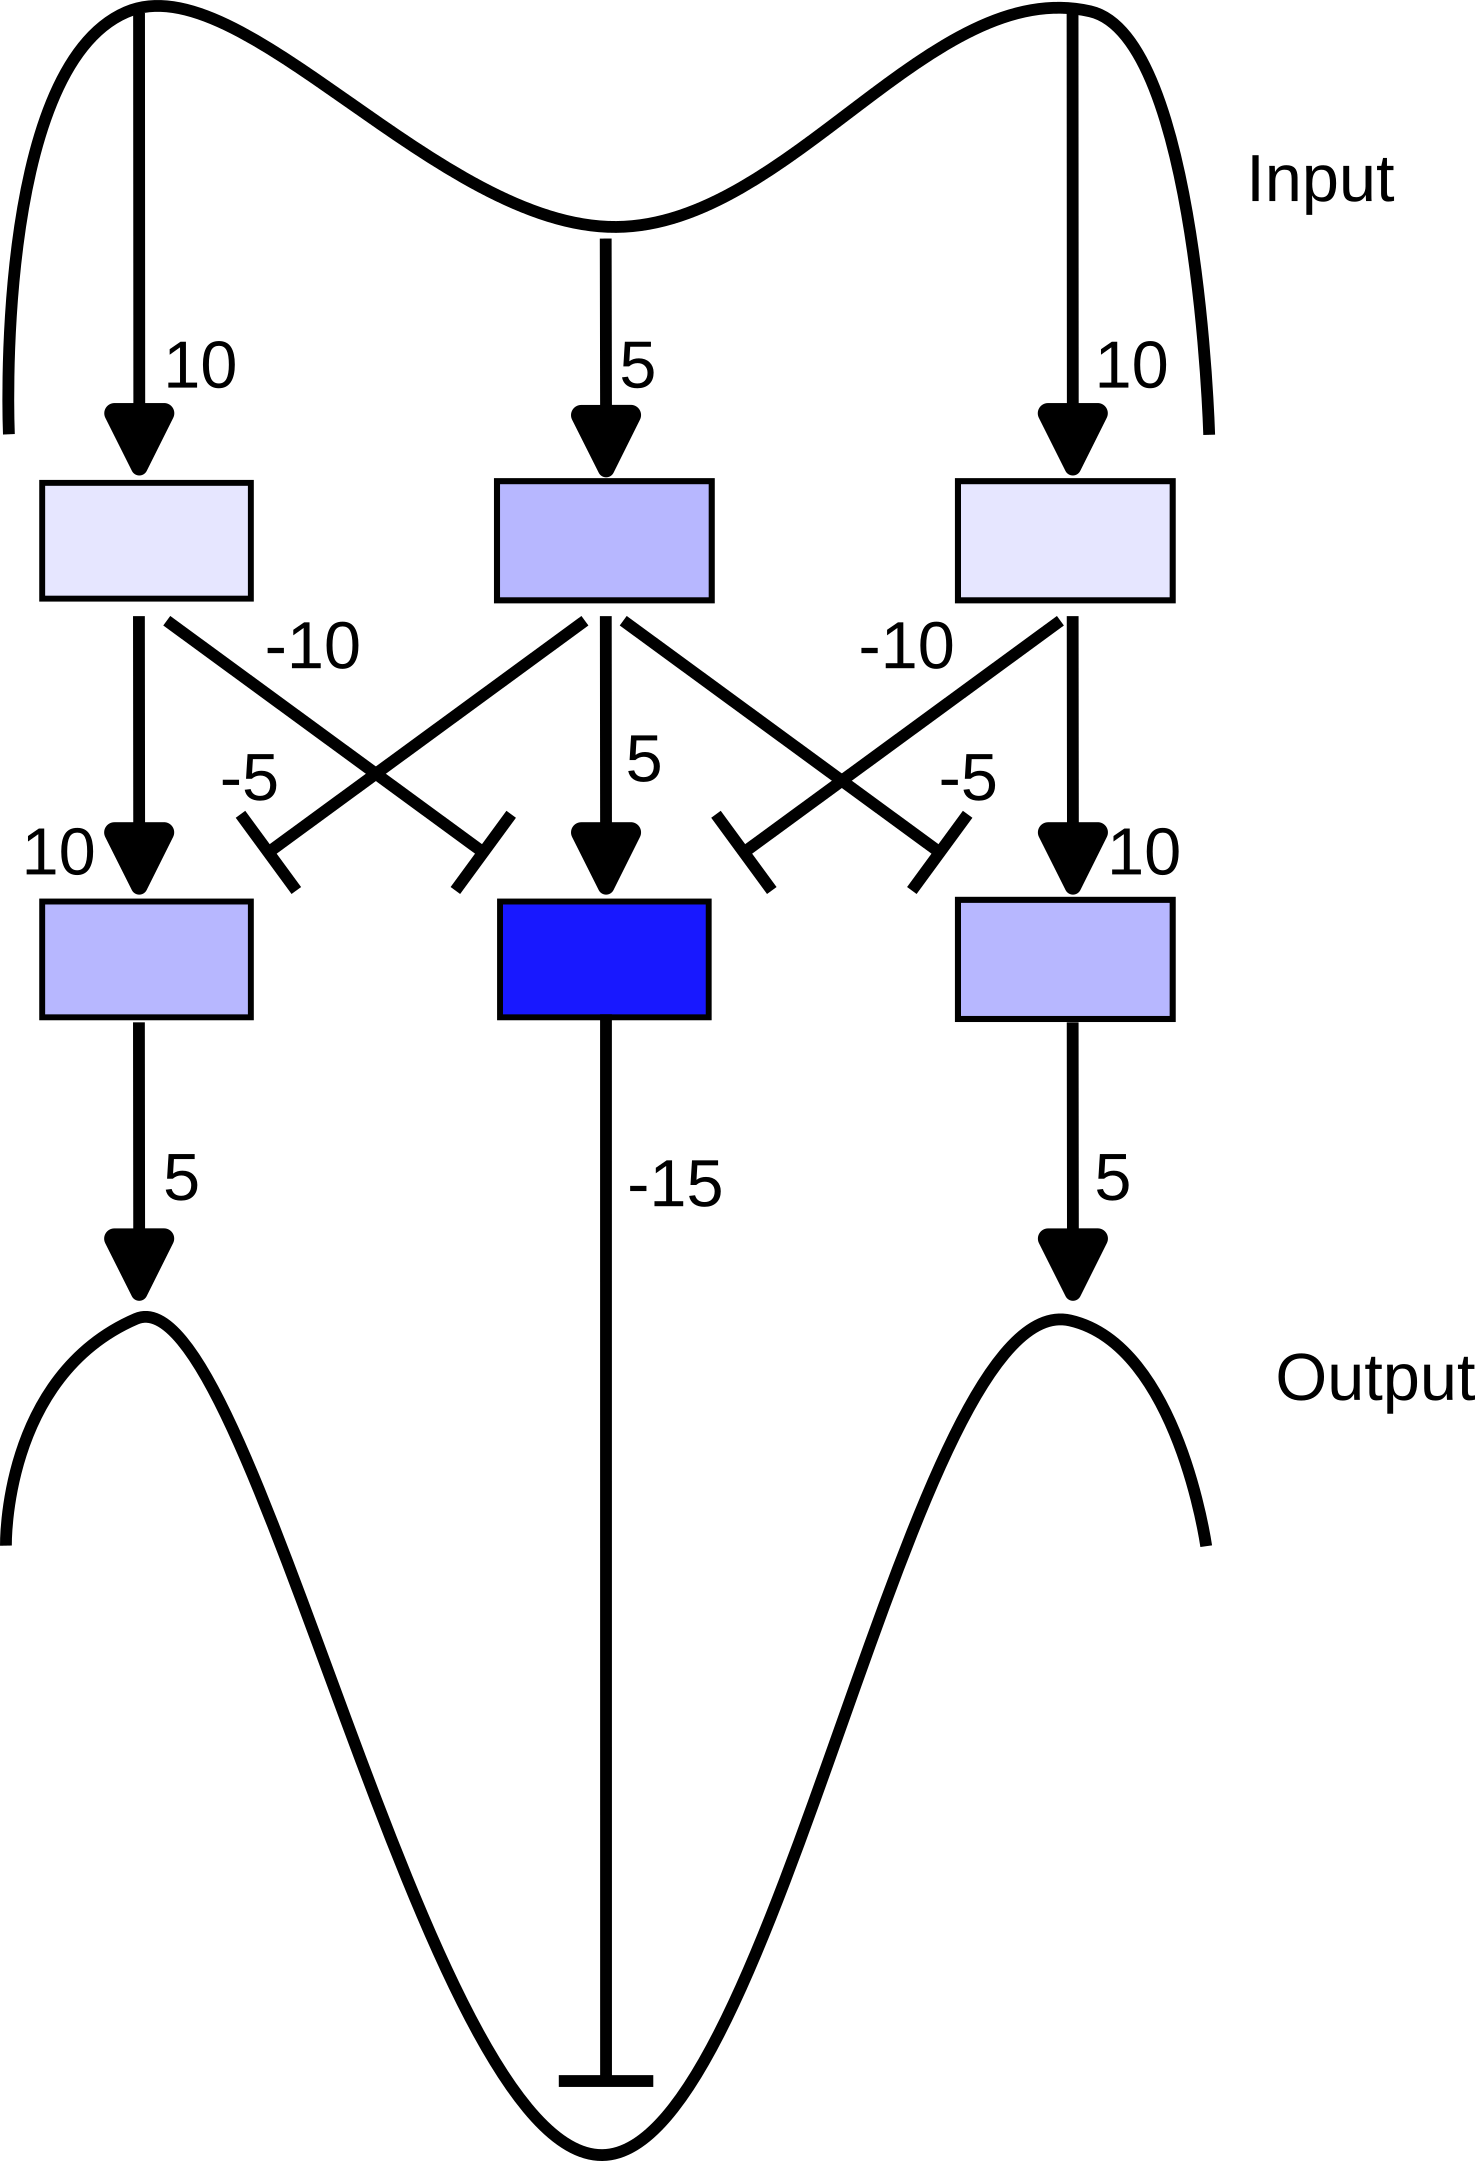
\includegraphics[width=0.301\textwidth]{laterale_hemmung.png}
\end{center}


\end{frame}

%% Sensorische Bahnen
\begin{frame}{Sensorische Bahnen}
\begin{center}
    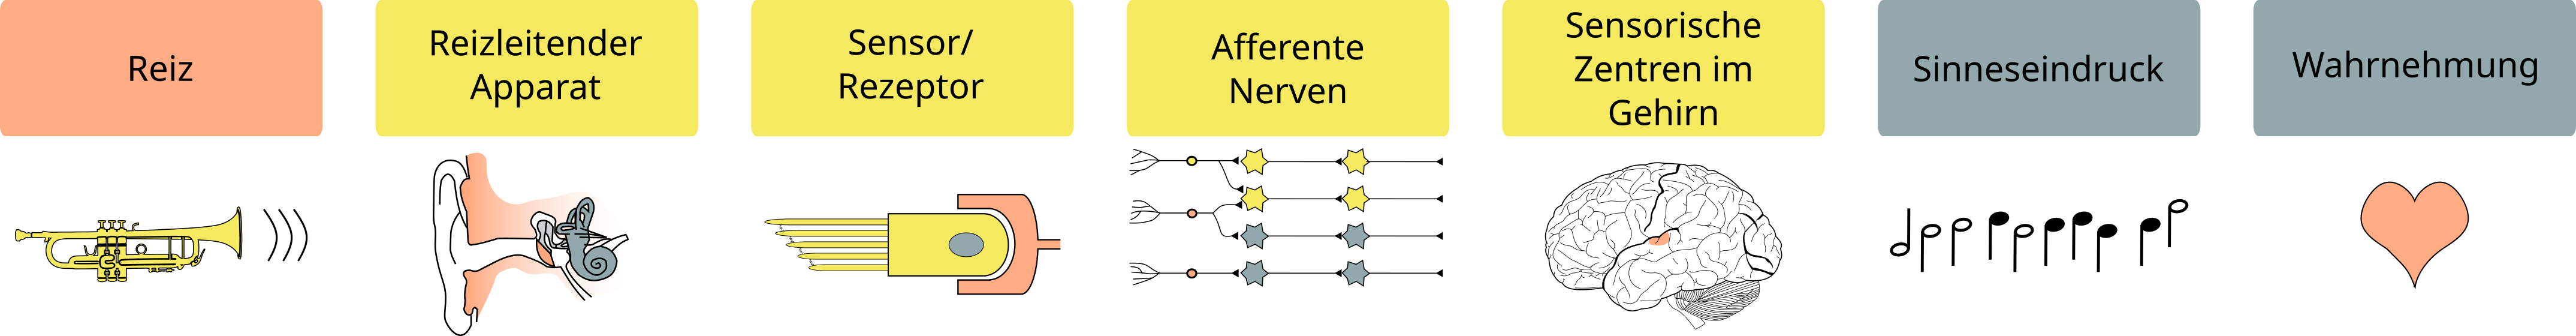
\includegraphics[width=\textwidth]{wahrnehmungsprozess.png}
\end{center}
    
\end{frame}



% Aufmerksamkeit, Bsp. Party 

\begin{frame}{Sensorische Bahnen}


\begin{columns}[c]

\begin{column}{7cm} 
Spezifische sensorische Bahnen gehen in spezialisierte Regionen je nach Sinnesmodalität (z.B. visueller Kortex beim Sehen)  \\[0.2 cm]

\pause

Zusätzlich gibt es unspezifische Bahnen vom Thalamus in alle Bereiche des Cortex (ARAS, Regulierung der Aufmerksamkeit). Beispiel: Unterhaltung auf einer Party trotz Hintergrund-Lärm

\end{column}

\begin{column}{5cm}
\begin{center}
    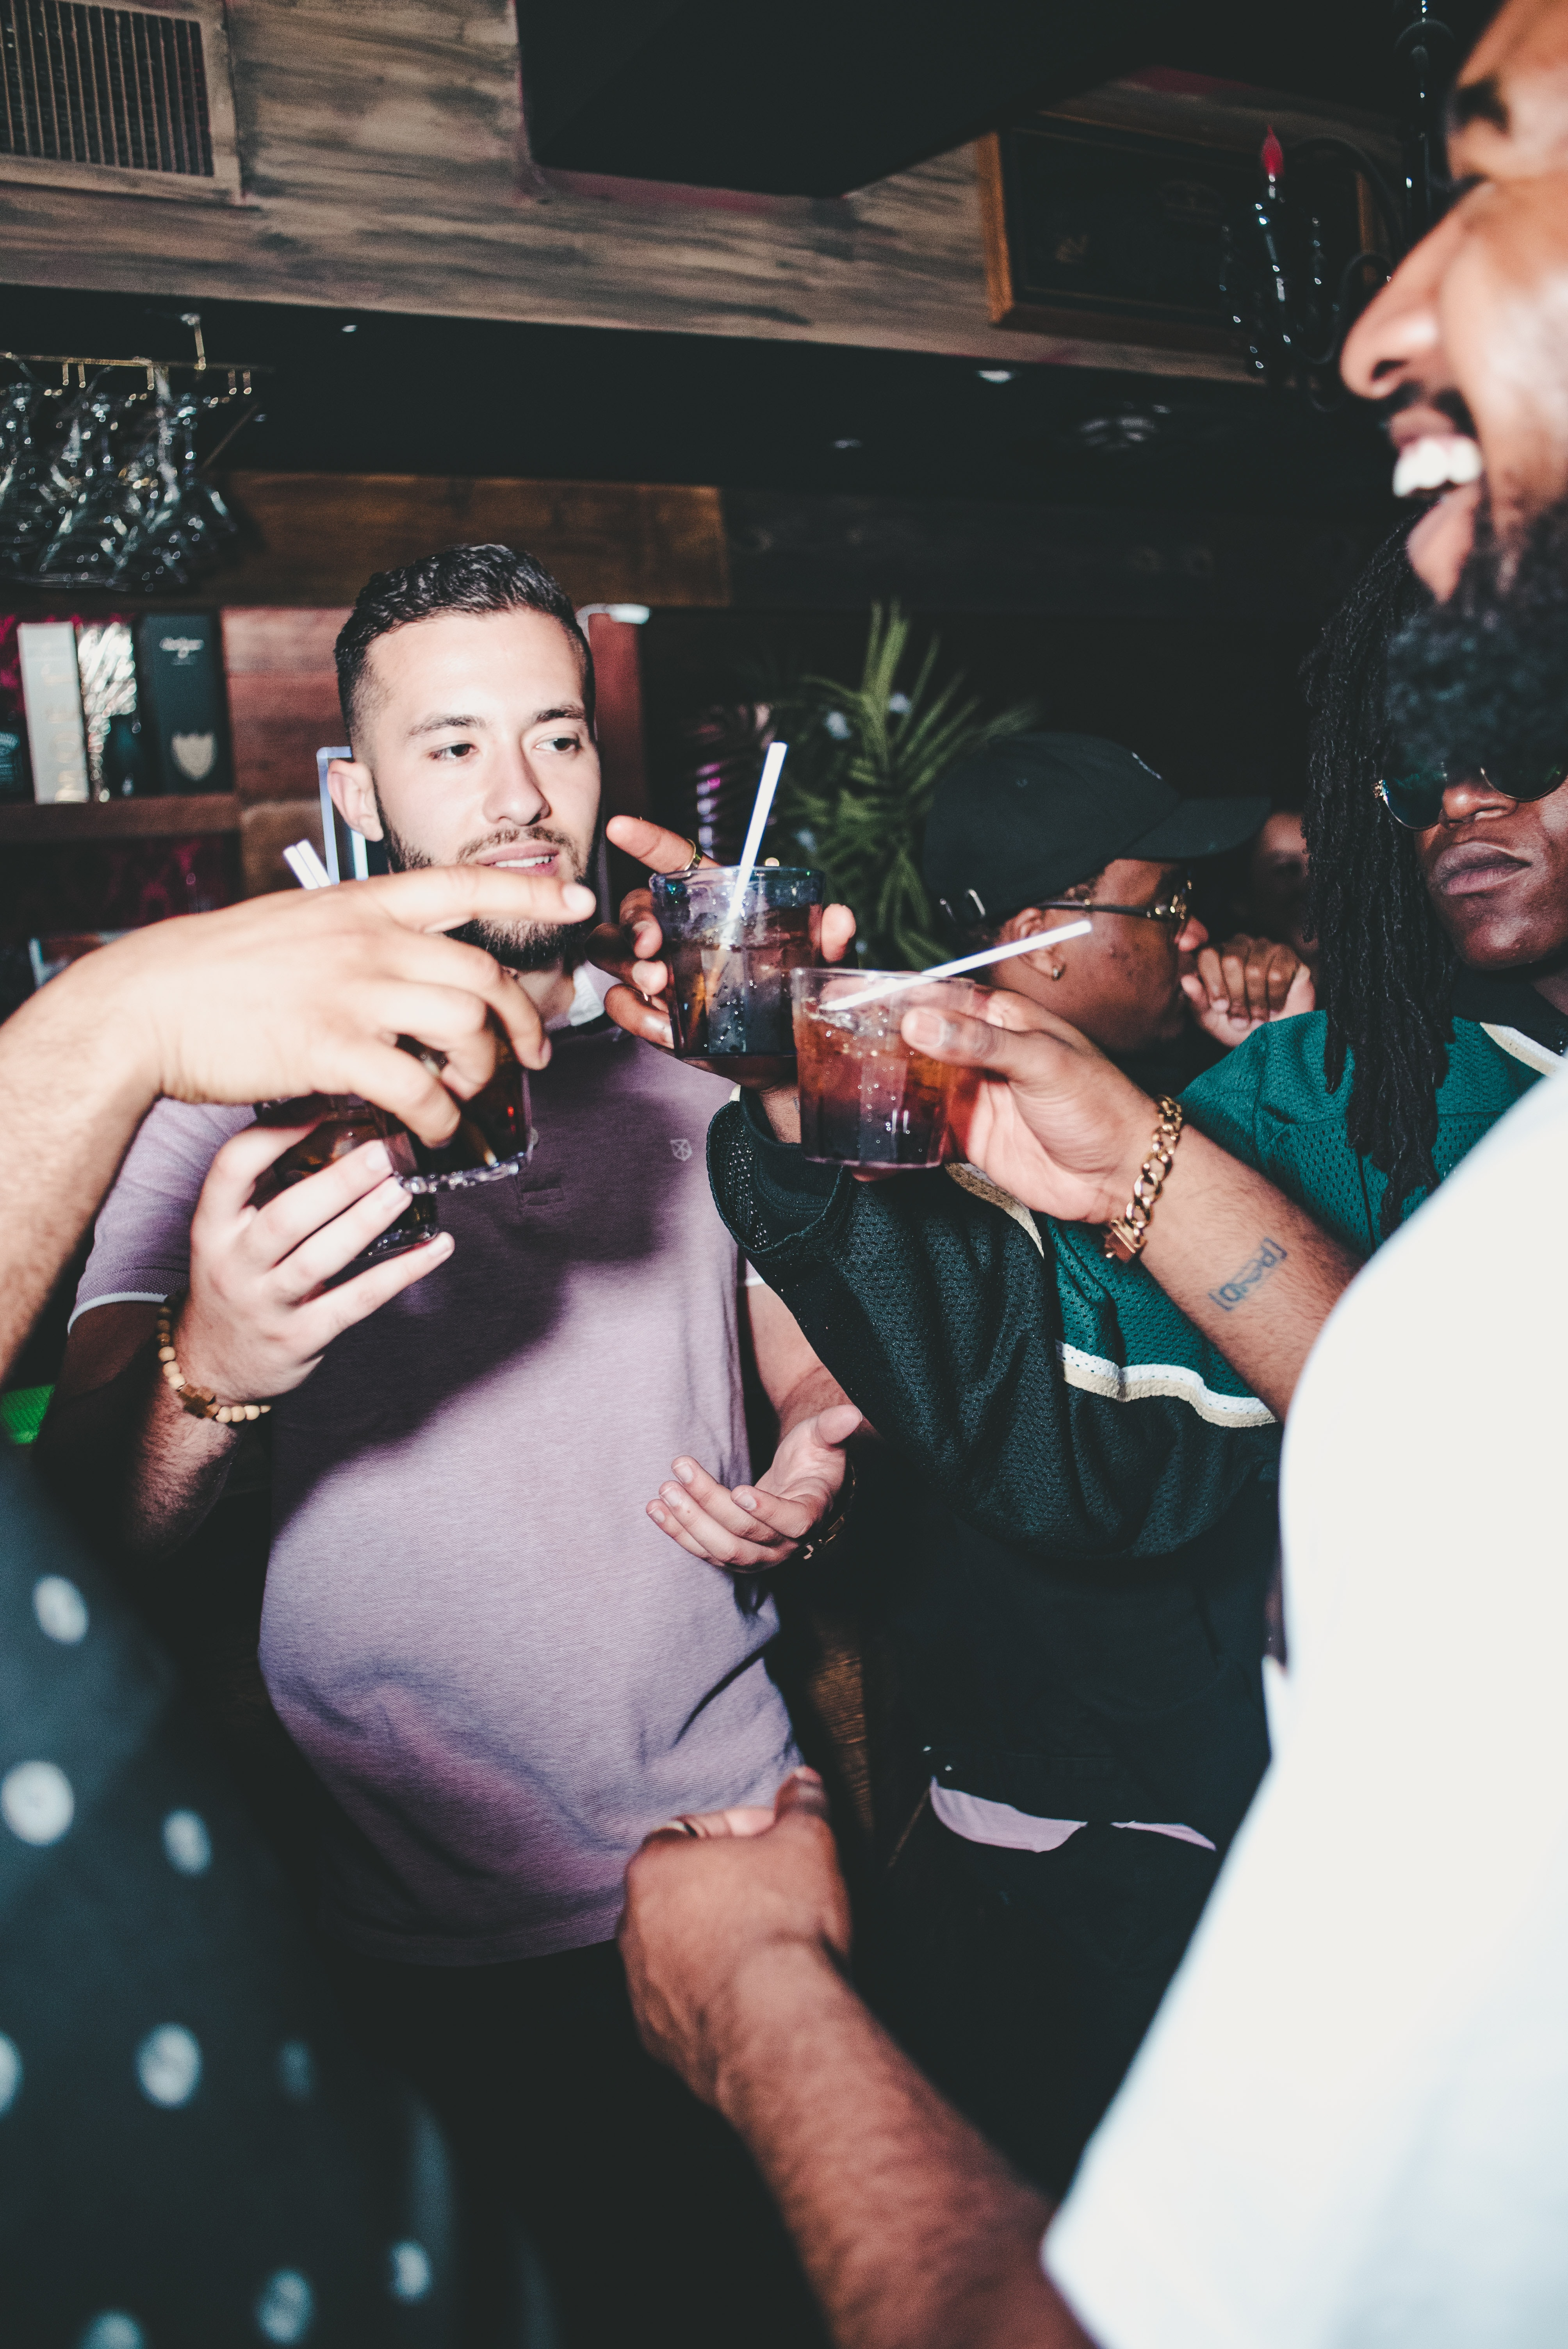
\includegraphics[width=\textwidth]{party.jpg}
\end{center}

\end{column}


\end{columns}







\end{frame}

%% Rolle von Erfahrung, Bsp. Agnosie, Bsp. The dress
\begin{frame}{Sensorische Bahnen}

Bereits vorhandenes Erfahrungswissen erlaubt es uns, Sinneseindrücke zu erkennen und zu klassifizieren. \\[1cm]

\pause

\begin{block}{Beispiel: Agnosie}

"Eine durchgehende Oberfläche [...], die eine Umhüllung bildet. [...] Sie scheint [...] fünf Ausstülpungen zu haben. [...] Eine Art Behälter? [...] Man könnte es zum Beispiel als Portemonnaie verwenden, für fünf verschiedene Münzgrößen." 

\begin{flushright}
Aus: Oliver Sacks.  \\ Der Mann, der seine Frau mit einem Hut verwechselte 
\end{flushright}
 

\end{block}




\end{frame}


%%% Spoiler alert
\begin{frame}{}

\begin{center}
    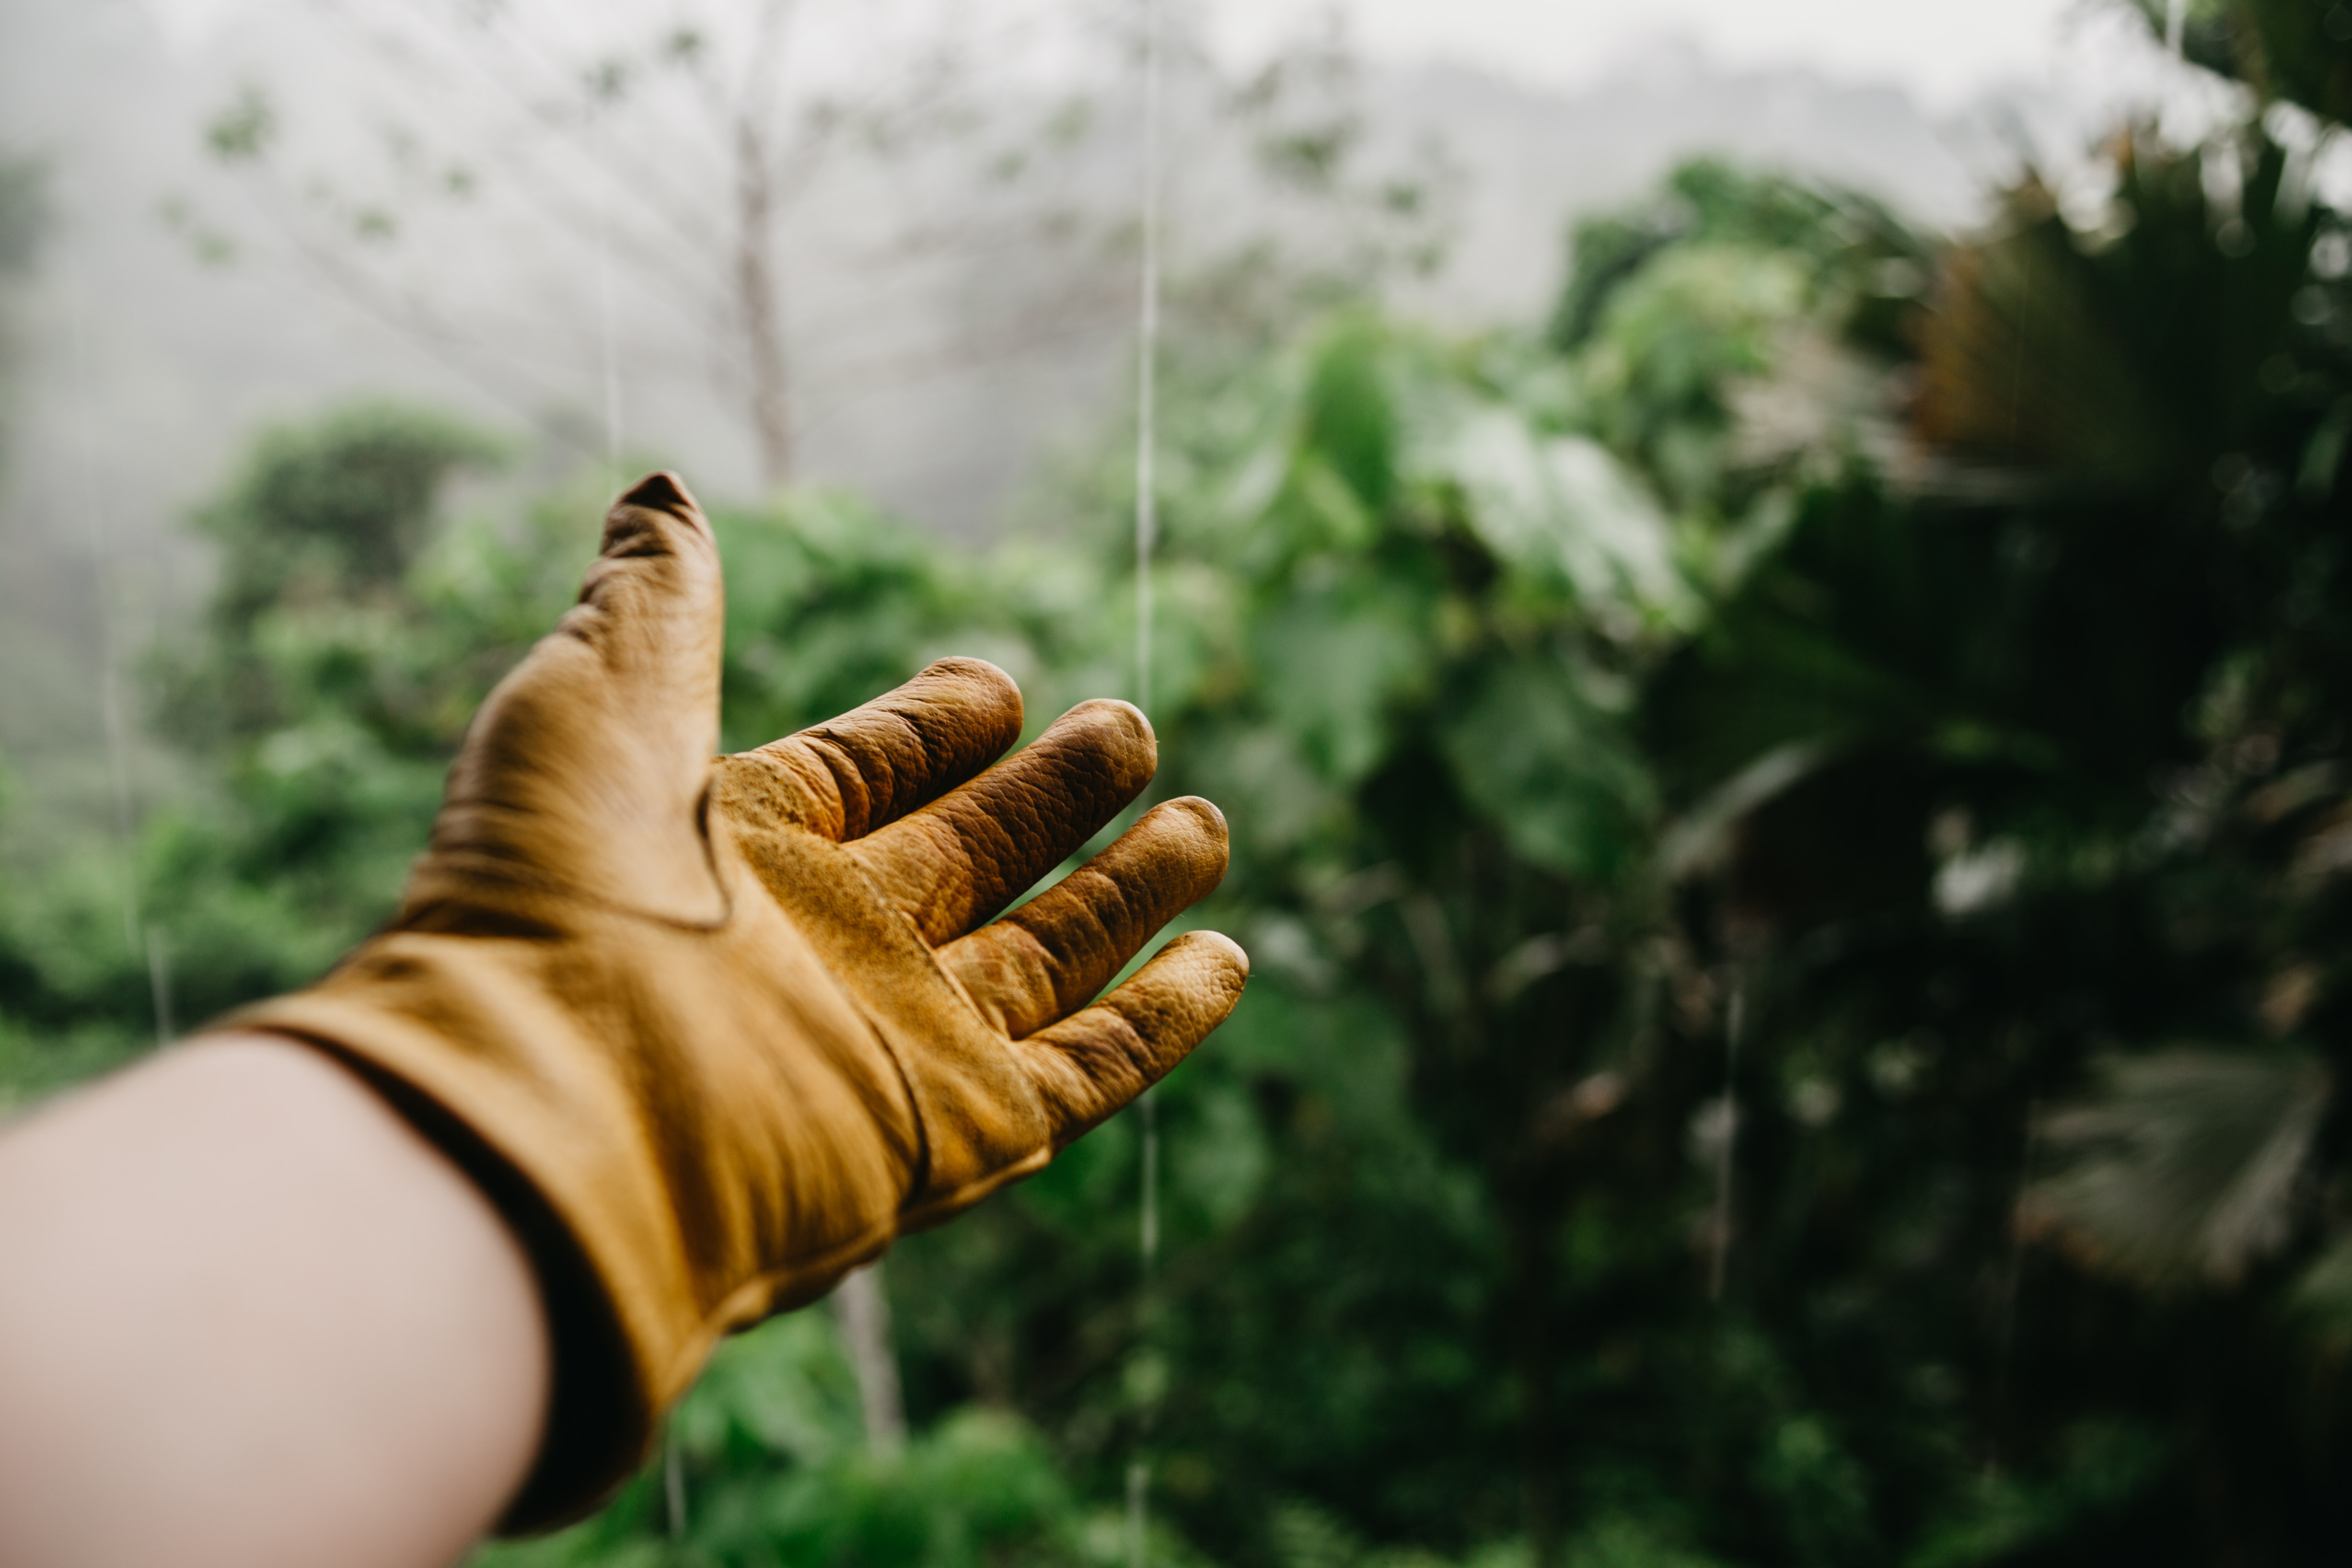
\includegraphics[width=\textwidth]{vince-fleming-7xcJsTrkvRc-unsplash.jpg}
\end{center}
    
\end{frame}
%%% 

\section{Woher wissen wir das?}

%% Was ist Psychophysik?
\begin{frame}{Psychophysik}

\begin{columns}[c]

\begin{column}{5cm}

Wissenschaft vom Zusammenhang zwischen äußeren Reizen und deren Empfindung und Wahrnehmung.


\end{column}


\begin{column}{5cm}
\begin{center}
    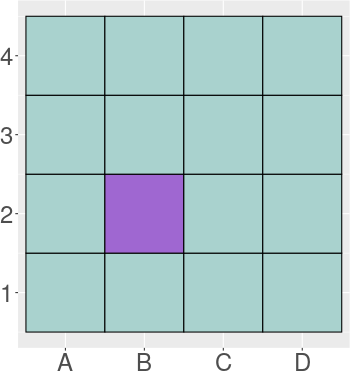
\includegraphics[width=\textwidth]{color_test_screenshot_3.png}
\end{center}
\end{column}


\end{columns}
    
\end{frame}

%% Reizschwellen
\begin{frame}{Reizschwellen}
Schwellenwerte bei der Wahrnehmung von Reizen.

\begin{itemize}
    \item 
\textbf{Wahrnehmungsschwelle/Absolutschwelle}: Kann ein Reiz überhaupt wahrgenommen werden? 
\pause
\item
\textbf{Erkennungsschwelle}: Kann der Reiz erkannt/benannt werden?

\pause
    \item
\textbf{Unterschiedsschwelle}: Können Reize voneinander unterschieden werden? \\[0.2 cm]

    \begin{columns}[c]
    
    \begin{column}{3.2cm}
    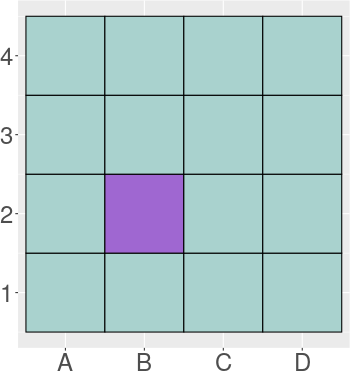
\includegraphics[width=\textwidth]{color_test_screenshot_3.png}
    
    \end{column}
    
    
    \begin{column}{3.2cm}
    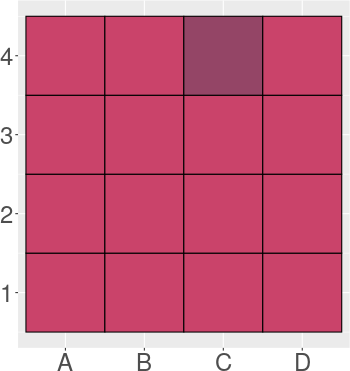
\includegraphics[width=\textwidth]{color_test_screenshot.png}
    
    \end{column}
    
    
    \begin{column}{3.2cm}
    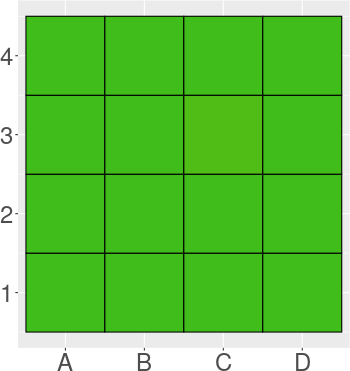
\includegraphics[width=\textwidth]{color_test_screenshot_2.png}
    
    \end{column}
    
\end{columns}

$\,$\\

\pause
    \item
\textbf{Sättigungsschwelle}: Kann eine Steigerung der Intensität noch wahrgenommen werden?
\pause
    \item
\textbf{Schmerzschwelle}: Wird der Reiz als schmerzhaft wahrgenommen?
\end{itemize}
    
    
\end{frame}


%% Bestimmung von Reizschwellen - incld. 2AFC
\begin{frame}{Wie können Reizschwellen bestimmt werden?}

\begin{center}
    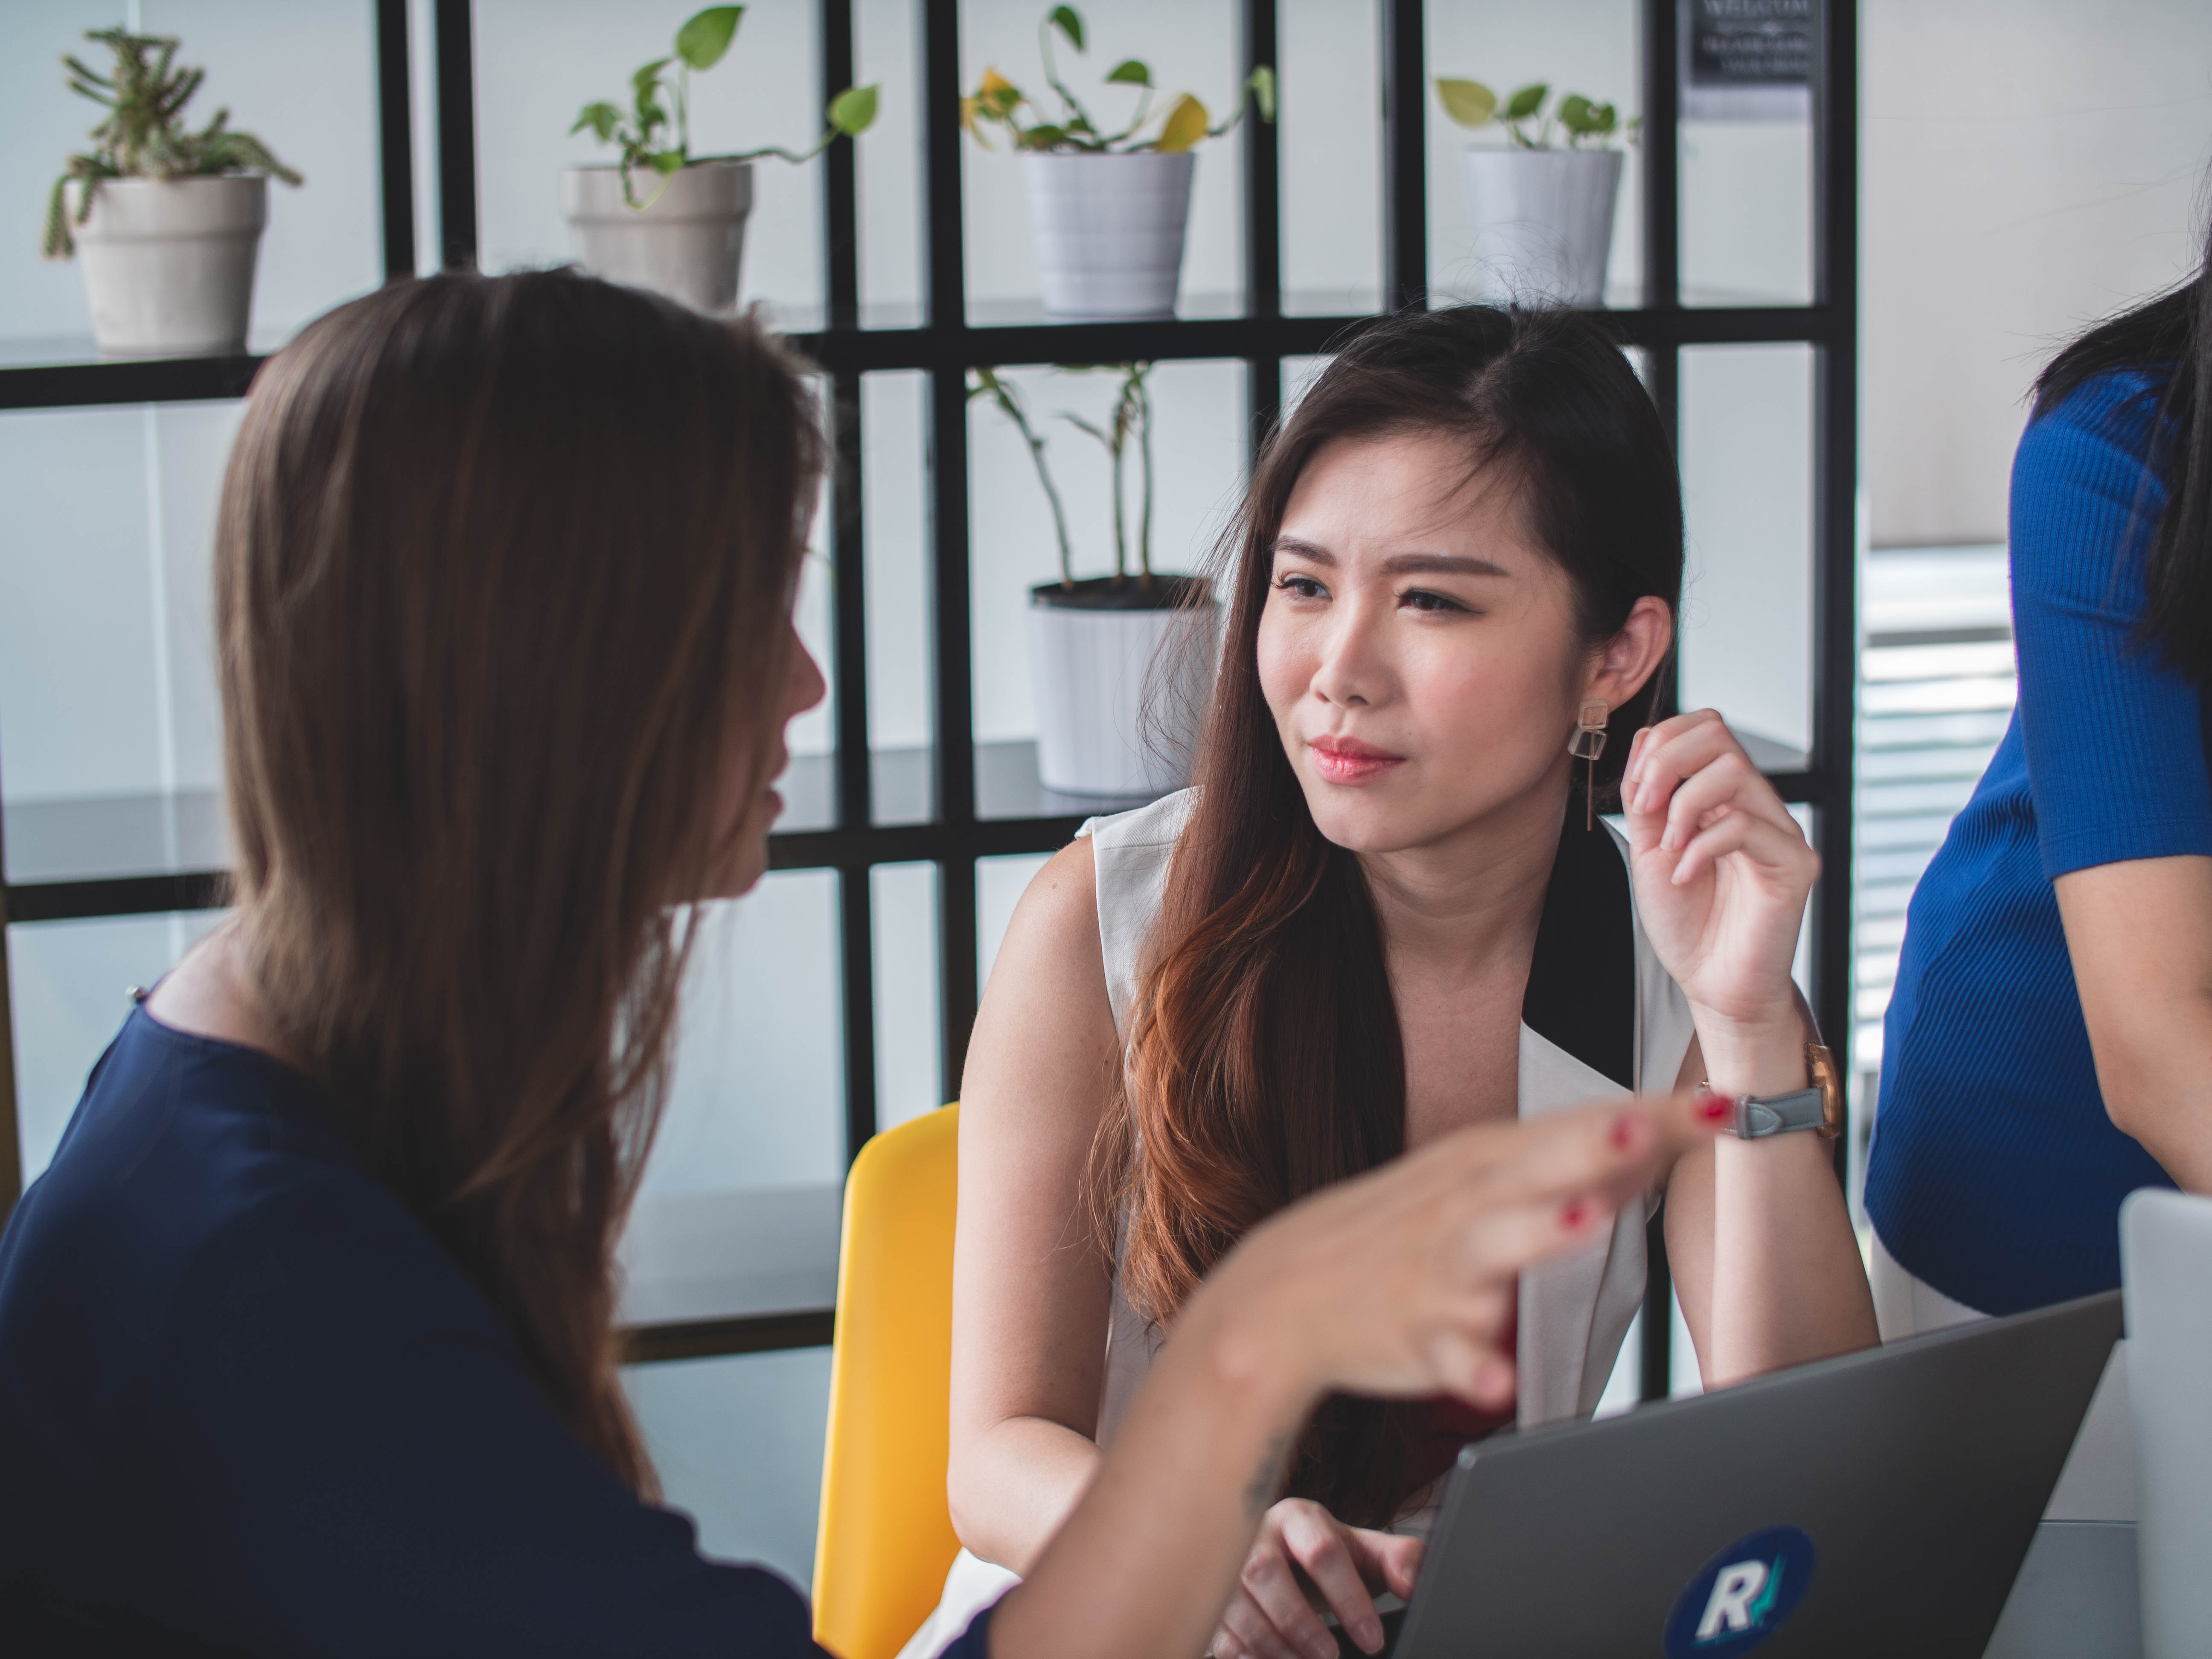
\includegraphics[width=\textwidth]{zweiergespraech.jpg}
\end{center}

    
\end{frame}



%% 
\begin{frame}{Reizschwellenbestimmung: Grenzmethode}


%%% Spoiler alert
\begin{center}
\includegraphics<1>[width=0.4\textwidth]{reizschwelle_seriell_1.png}
\includegraphics<2>[width=0.4\textwidth]{reizschwelle_seriell_2.png}
\includegraphics<3>[width=0.4\textwidth]{reizschwelle_seriell_3.png}
\includegraphics<4>[width=0.4\textwidth]{reizschwelle_seriell_4.png}
\includegraphics<5>[width=0.4\textwidth]{reizschwelle_seriell_5.png}
\includegraphics<6>[width=0.4\textwidth]{reizschwelle_seriell_6.png}
\includegraphics<7>[width=0.4\textwidth]{reizschwelle_seriell_7.png}
\includegraphics<8>[width=0.4\textwidth]{reizschwelle_seriell_8.png}
\includegraphics<9>[width=0.4\textwidth]{reizschwelle_seriell_9.png}
\includegraphics<10>[width=0.4\textwidth]{reizschwelle_seriell_10.png}
\end{center}

    
\end{frame}



\begin{frame}{Reizschwellenbestimmung}

\begin{itemize}
    \item 
    Grenzmethode: Reiz wird schrittweise erhöht oder verringert. Versuchsperson sagt, ob sie den Reiz wahrnehmen kann.
    
\end{itemize}

\end{frame}



\begin{frame}{Reizschwellenbestimmung: Konstanzmethode}


\begin{center}

\includegraphics<1>[width=0.4\textwidth]{reizschwelle_seriell_2.png}
\includegraphics<2>[width=0.4\textwidth]{reizschwelle_seriell_5.png}
\includegraphics<3>[width=0.4\textwidth]{reizschwelle_seriell_8.png}
\includegraphics<4>[width=0.4\textwidth]{reizschwelle_seriell_6.png}
\includegraphics<5>[width=0.4\textwidth]{reizschwelle_seriell_1.png}
\includegraphics<6>[width=0.4\textwidth]{reizschwelle_seriell_10.png}
\includegraphics<7>[width=0.4\textwidth]{reizschwelle_seriell_3.png}

\end{center}

    
\end{frame}



\begin{frame}{Reizschwellenbestimmung}

\begin{itemize}
    \item 
    Grenzmethode: Reiz wird schrittweise erhöht oder verringert. Versuchsperson sagt, ob sie den Reiz wahrnehmen kann.
    \item
    Konstanzmethode: Reize werden in zufälliger Reihenfolge präsentiert. Versuchsperson sagt, ob sie den Reiz wahrnehmen kann.
    
\end{itemize}

\end{frame}




%% 2AFC
\begin{frame}{Reizschwellenbestimmung: 2-Alternative Forced Choice Methode}


\begin{center}


\includegraphics<1>[width=0.4\textwidth]{reizschwelle_seriell_8.png}
\includegraphics<2>[width=\textwidth]{reizschwelle_AFC_3.png}
\includegraphics<3>[width=\textwidth]{reizschwelle_AFC_1.png}
\includegraphics<4>[width=0.4\textwidth]{reizschwelle_seriell_4.png}
\includegraphics<5>[width=0.4\textwidth]{reizschwelle_seriell_10.png}
\includegraphics<6>[width=0.4\textwidth]{reizschwelle_seriell_1.png}
\includegraphics<7>[width=\textwidth]{reizschwelle_AFC_2.png}

\end{center}

    
\end{frame}


%% end spoiler alert


%% Zusammenfassung Methoden
\begin{frame}{Reizschwellenbestimmung}

\begin{itemize}
    \item 
    Grenzmethode: Reiz wird schrittweise erhöht oder verringert. Versuchsperson sagt, ob sie den Reiz wahrnehmen kann.
    \item
    Konstanzmethode: Reize werden in zufälliger Reihenfolge präsentiert. Versuchsperson sagt, ob sie den Reiz wahrnehmen kann.
    \item
    2-Alternative Forced Choice: Versuchsperson* muss den Reiz benennen (aus einer Auswahl von zwei) 
\end{itemize}

\end{frame}


%% Reizschwellenbestimmung: Auswertung



\begin{frame}{Reizschwellenbestimmung: Auswertung}

\begin{center}
    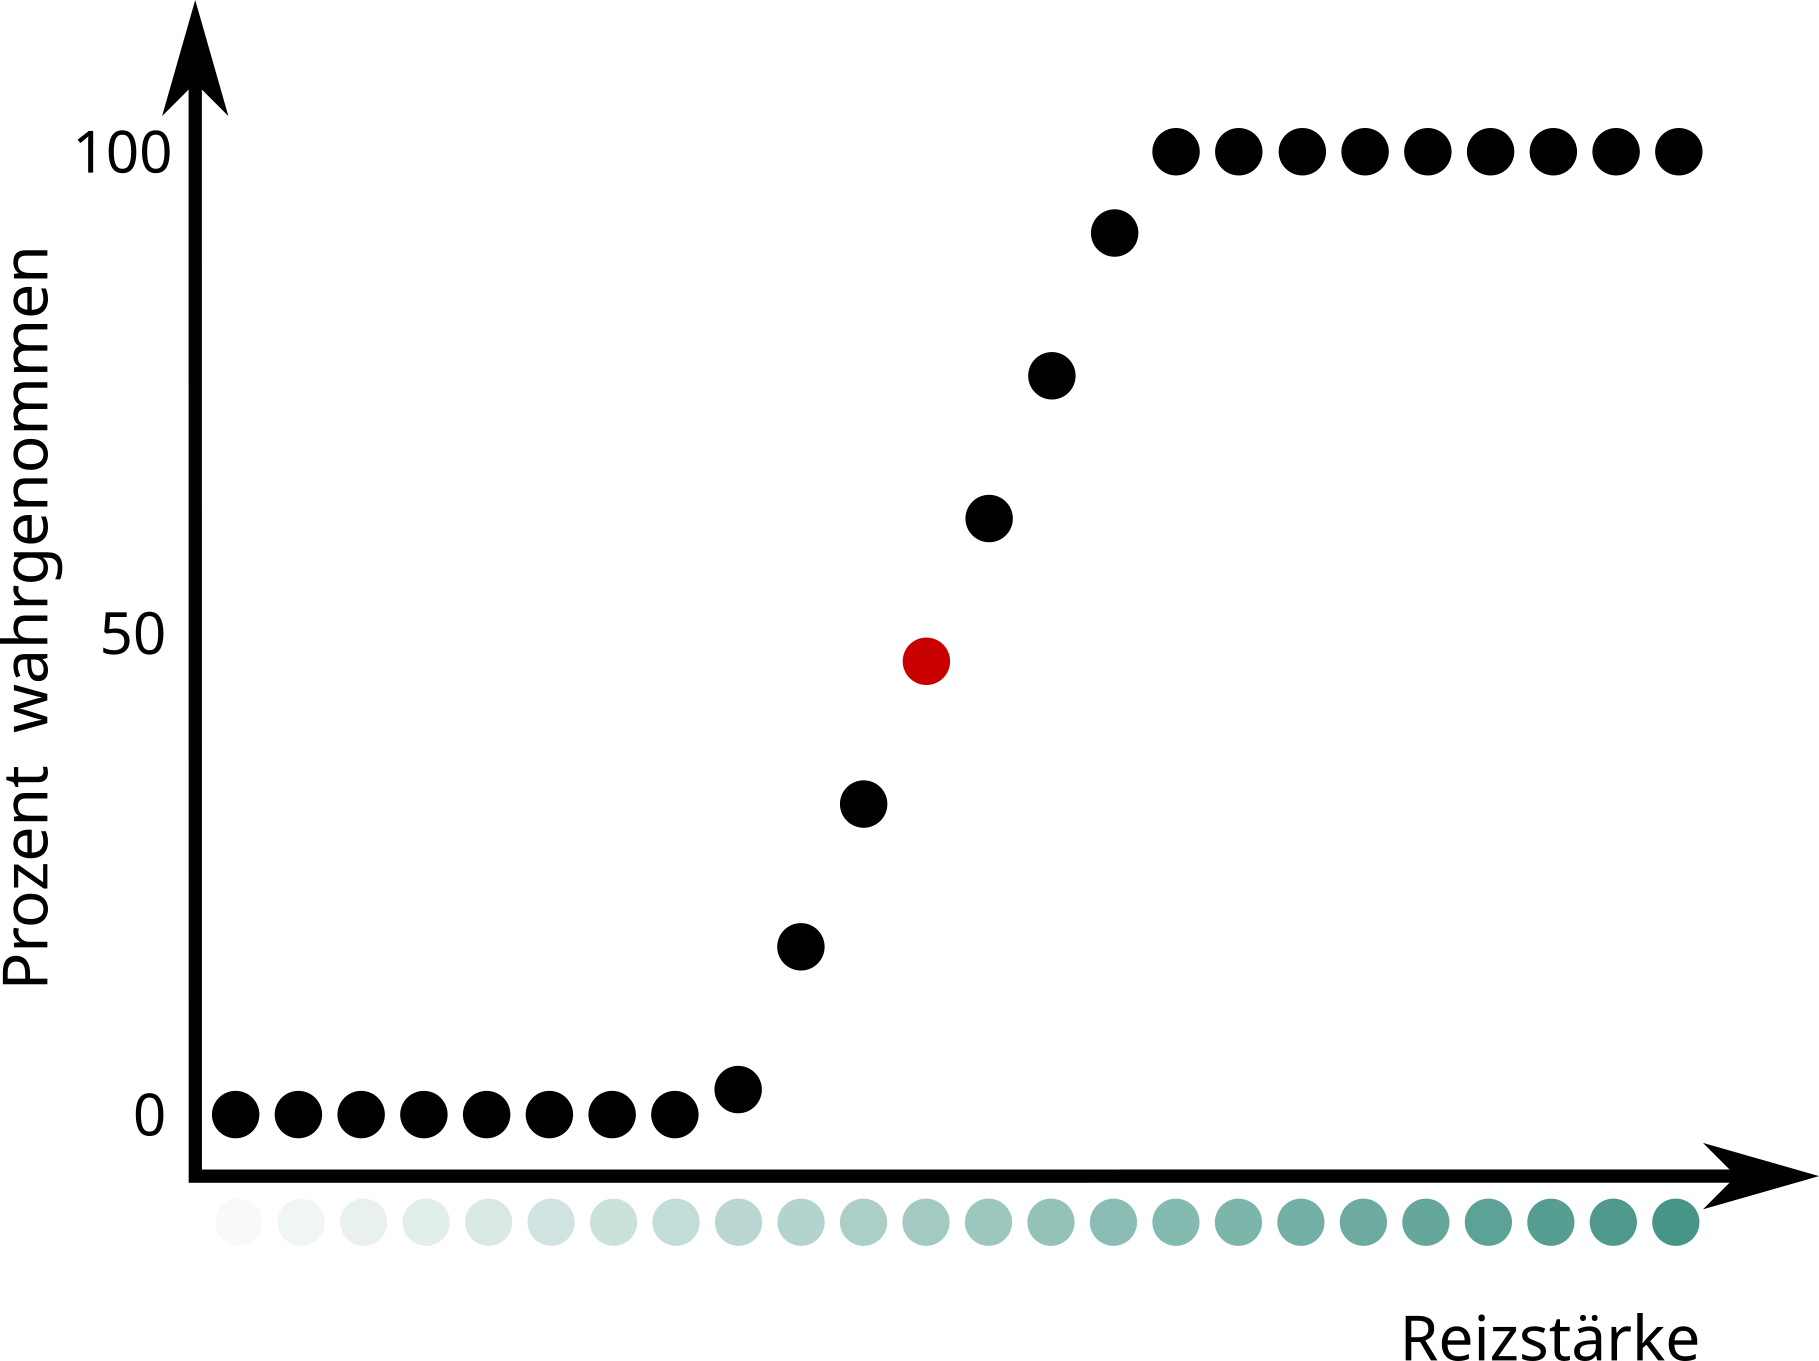
\includegraphics[width=0.8\textwidth]{reizschwellen_diagramm.png}
\end{center}

\end{frame}


%% Weber-Fechner


%% Motivation: Apfel
\begin{frame}{Was für Unterschiede können wir eigentlich wahrnehmen?}

Ein Apfel wiegt ca. \SI{150}{\gram}. Können Sie diesen Gewichtsunterschied wahrnehmen? 


\begin{center}
    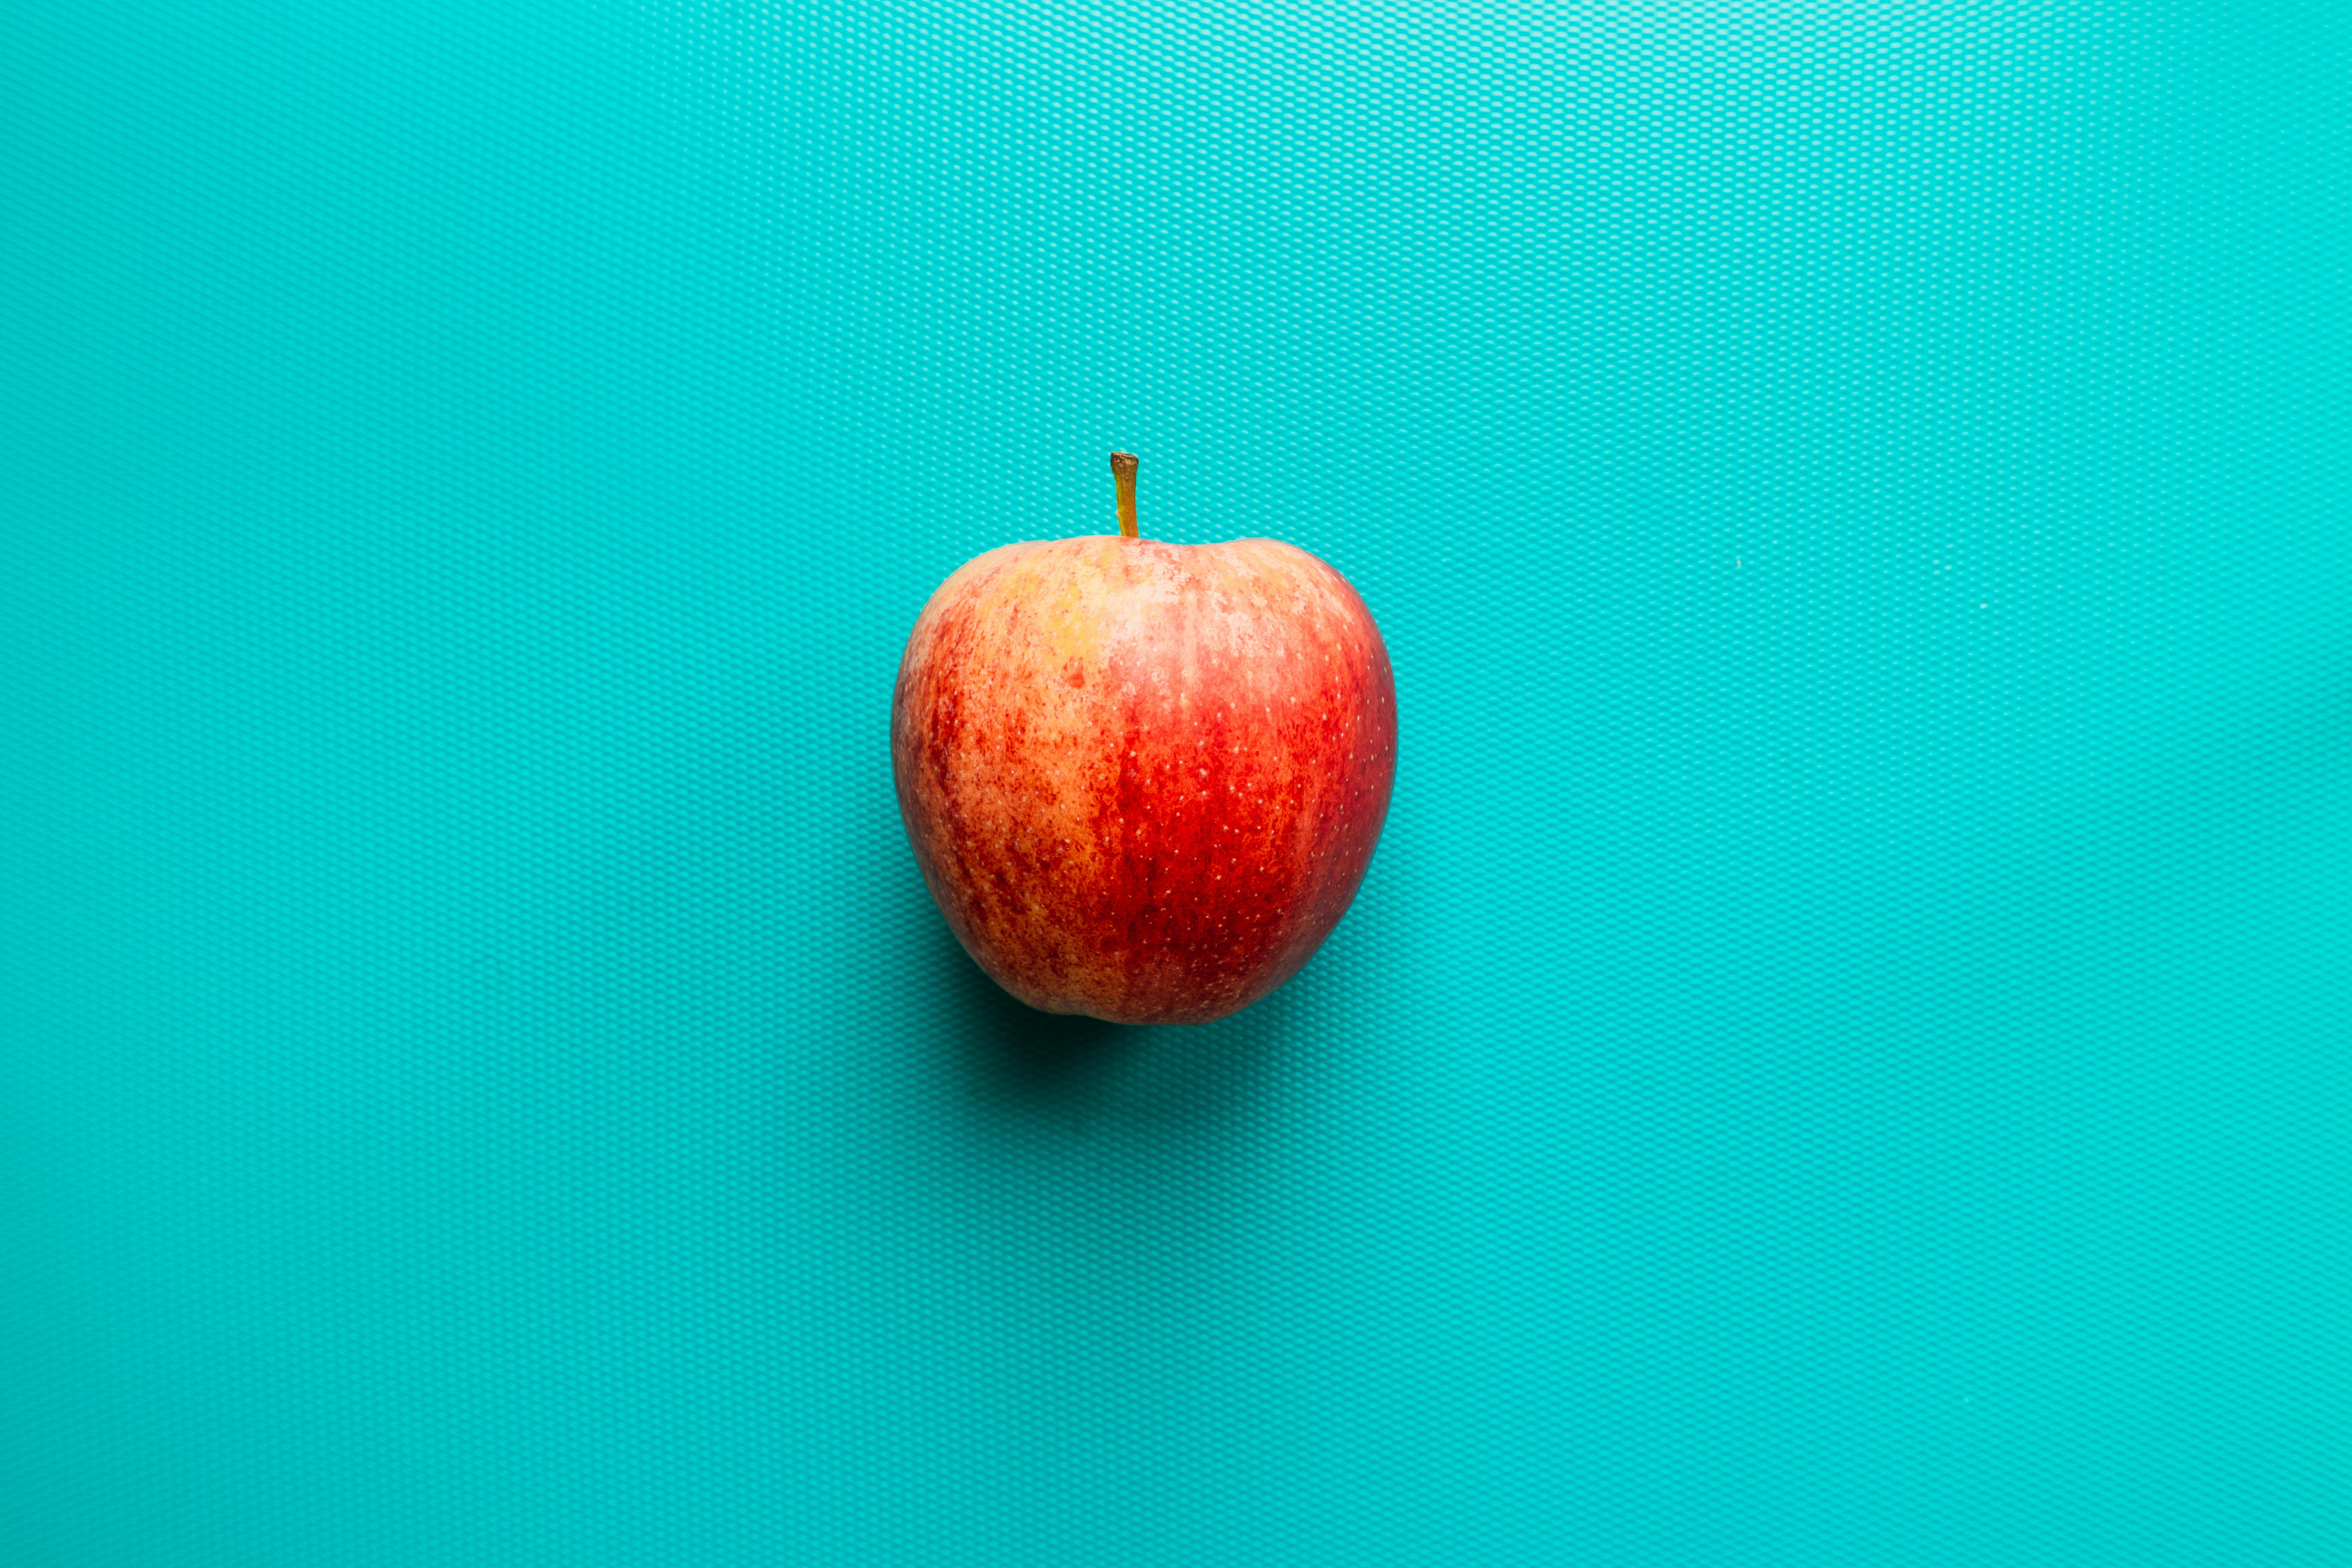
\includegraphics[width=0.8\textwidth]{louis-hansel-MardkT836BU-unsplash.jpg}
    
\end{center}

    
\end{frame}


%% Apfel: Kommt drauf an
\begin{frame}{Was für Unterschiede können wir eigentlich wahrnehmen?}

Kommt drauf an \dots

\begin{center}
    \includegraphics<1>[width=0.8\textwidth]{priscilla-du-preez-CoqJGsFVJtM-unsplash.jpg}
        \includegraphics<2>[width=0.8\textwidth]{liuba-bilyk-wU_TbWqdPJI-unsplash.jpg}

\end{center}

    
\end{frame}



%% Weber
\begin{frame}{Webersches Gesetz}

\[
\frac{\Delta R}{R} = k
\]

\[
\begin{array}{lll}
\Delta R    & \ldots    & \text{kleinster wahrnehmbarer Unterschied} \\
R           & \ldots    & \text{Reizstärke} \\
k           & \ldots    & \text{irgendeine Konstante*} \\
\end{array}
\]


(*\(k\) hängt von der Reizmodalität ab, ist aber innerhalb einer Reizmodalität konstant.)

\pause

\begin{block}{Auf Deutsch}
Der Unterschied, den wir noch feststellen können hängt davon ab, wie groß der Reiz eh schon ist. 
\end{block}



\end{frame}


\begin{frame}{Webersches Gesetz}
\begin{center}
    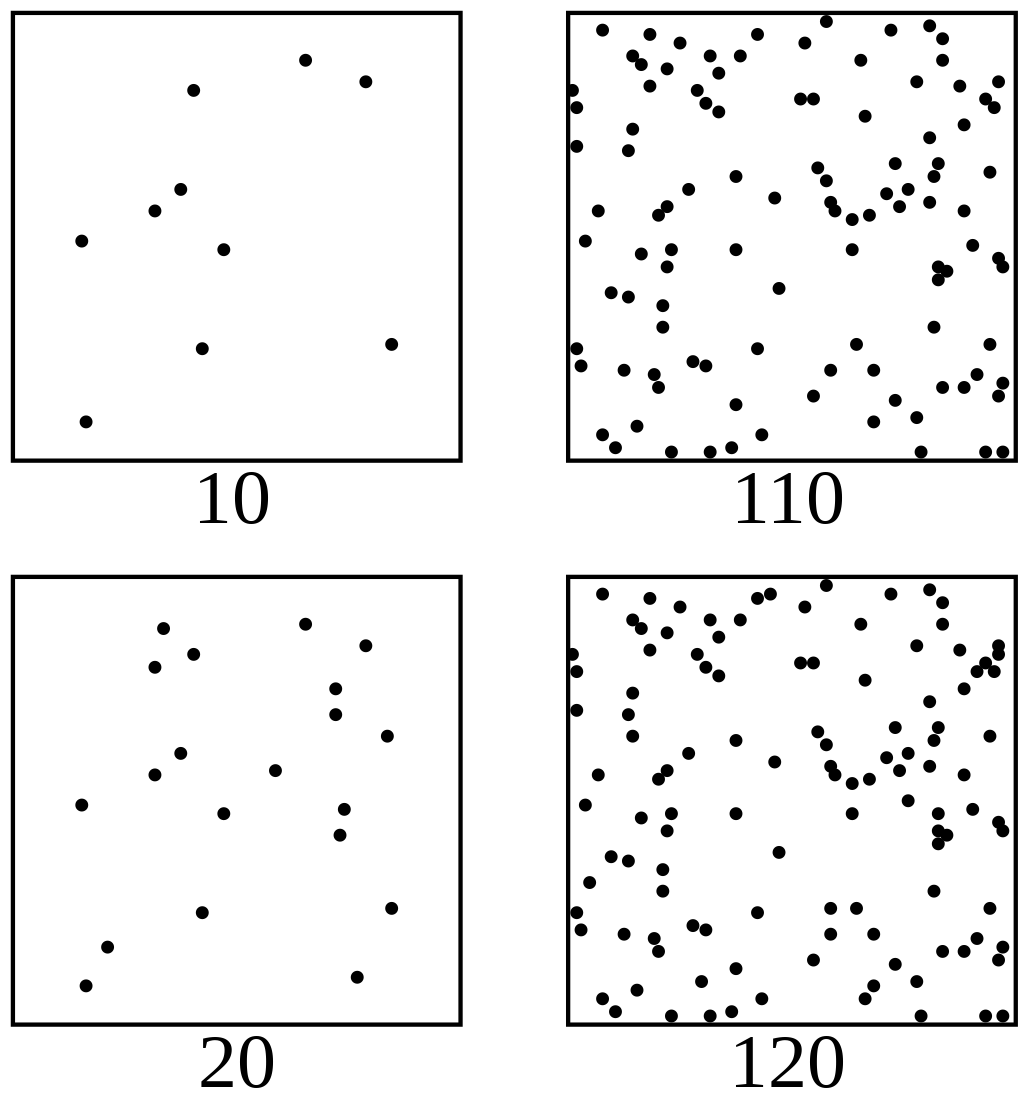
\includegraphics[width=0.6\textwidth]{Weber-Fechner_law_demo_-_dots.svg.png}
\end{center}
\end{frame}


%% Weber-Fechner
%% Inkscape plots started to illustrate Weber to Weber-Fechner
\begin{frame}{Webersches Gesetz}

\begin{center}
    \includegraphics<1>[width=0.8\textwidth]{weber_fechner_1.png}
    \includegraphics<2>[width=0.8\textwidth]{weber_fechner_2.png}
    \includegraphics<3>[width=0.8\textwidth]{weber_fechner_3.png}
\end{center}
    
\end{frame}


\begin{frame}{Gesetz von Weber und Fechner}

\begin{center}
    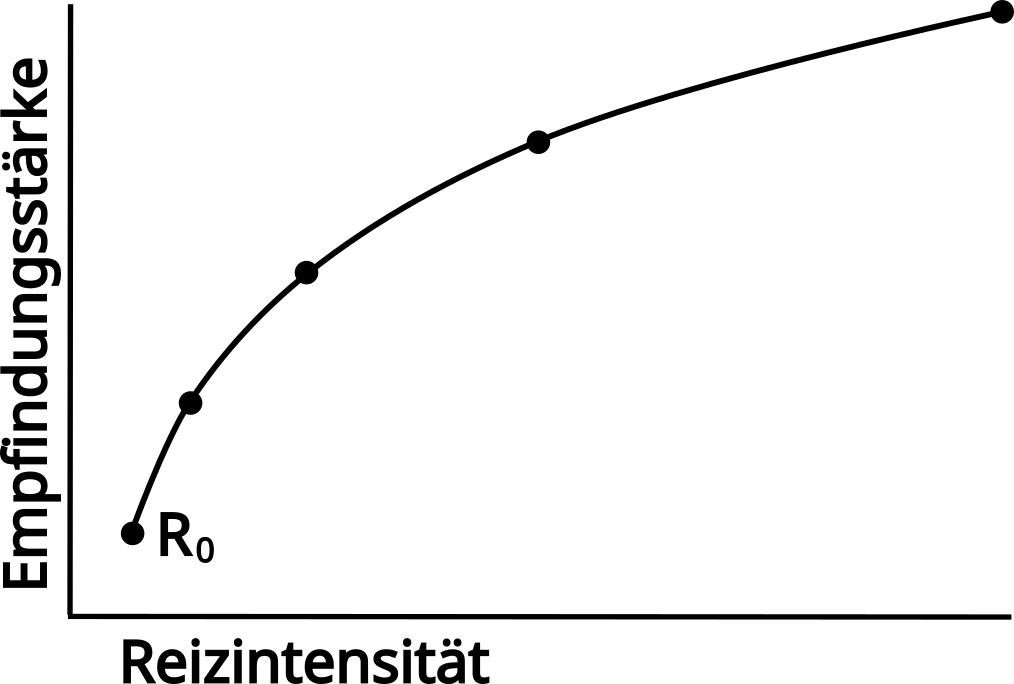
\includegraphics[width=0.8\textwidth]{weber_fechner.png}
\end{center}
    


\end{frame}


\begin{frame}{Gesetz von Weber und Fechner}

\[
E = c\log \frac{R}{R_0}
\]


\[
\begin{array}{lll}
E           &\ldots    & \text{Empfindungsstärke} \\
R           & \ldots    & \text{Reizstärke} \\
R_0           & \ldots    & \text{Reizschwelle} \\
c           & \ldots    & \text{irgendeine Konstante} \\
\end{array}
\]

\begin{block}{Auf Deutsch}
Die Empfindungsstärke hängt logarithmisch von der Reizintensität ab.
\end{block}

 
\end{frame}




% %% Beispiel: Dezibel
\begin{frame}{Gesetz von Weber und Fechner}

Kleines Physik-Flashback: Ein Dezibel sind 0.1 Bel. Aber was ist ein Bel? 

\pause

\[
\text{Schallstärke in Bel} = \lg \frac{\text{Schallstärkepegel}}{\text{Vergleichspegel}} 
\]

\pause

Vergleiche: 

\[
E = c\log \frac{R}{R_0}
\]


    
\end{frame}



%% Stevens

\begin{frame}{Wie können wir subjektive Wahrnehmung quantifizieren?}


Die Gesetze von Weber und Fechner befassen sich mit \textbf{Unterscheidbarkeit} von Reizen. Aber was, wenn wir nicht an Unterschieden interessiert sind, sondern nur daran, wie laut/schwer/hell/warm/etc. sich etwas anfühlt? 

\pause

There is a formula for that. 

\begin{center}
    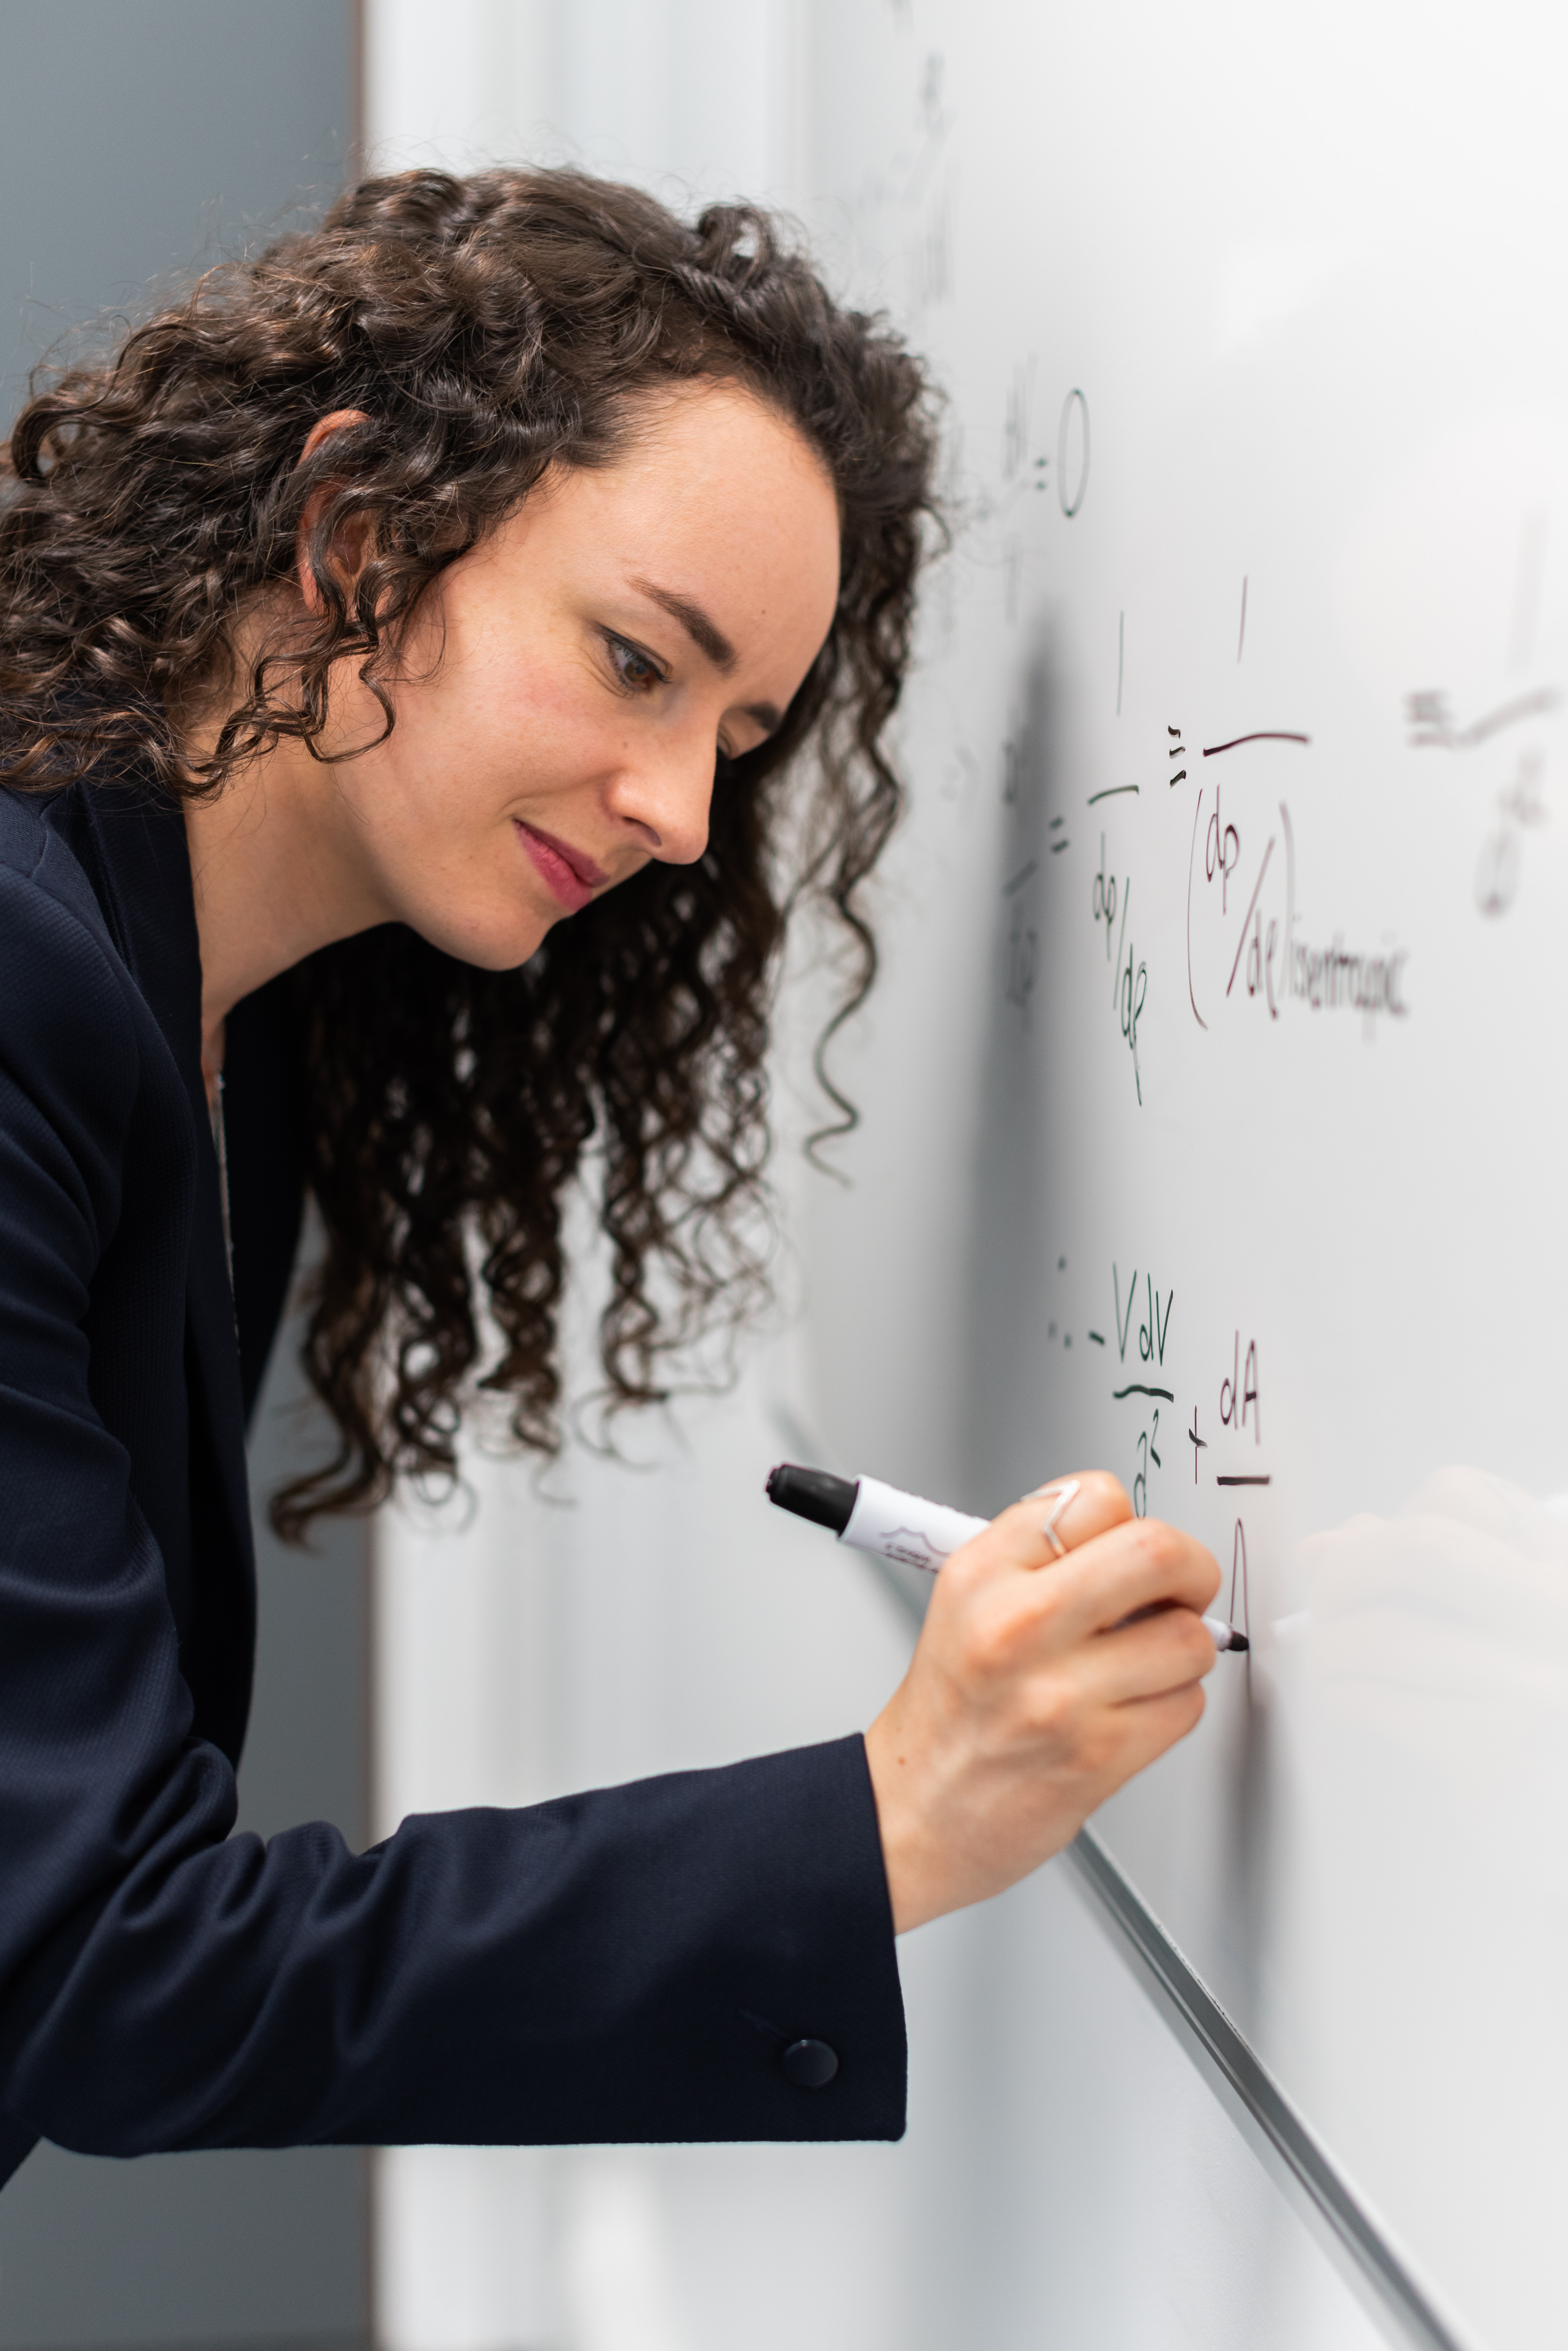
\includegraphics[width=0.4\textwidth]{thisisengineering-raeng-fgdmH3iqvMw-unsplash.jpg}
\end{center}


\end{frame}



\begin{frame}{Potenzfunktion von Stevens}

\[
E=k\cdot \left(R-R_{0}\right)^{n}
\]

\[
\begin{array}{lll}
E           &\ldots    & \text{Empfindungsstärke} \\
R           &\ldots    & \text{Reizstärke} \\
R_0           & \ldots    & \text{Reizschwelle} \\
k, n           & \ldots    & \text{irgendwelche Konstanten} \\
\end{array}
\]

\pause

\(n<1\): Zunahme der Reizantwort ist weniger stark als Zunahme des Reizes (ähnlich wie beim Weber-Fechner-Gesetz).  \\[0.2cm]



\(n=1\): Reizantwort ist proportional zum Reiz. \\[0.2 cm]

\(n>1\): Reizantwort wächst stärker als der Reiz. 



\end{frame}



%%% IMPP Frage 
%% Physio-Fragen Frage 525, image saved on iphone
\begin{frame}{IMPP Frage}


\begin{columns}[c]
\begin{column}{6cm}
Die Kenntnis der relativen Empfindlichkeit von Sinnessystemen spielt in der klinischen Diagnostik eine große Rolle. 

Welche der folgenden Abbildungen zeigt in diesem Zusammenhang am besten die Beziehung zwischen notwendigem Reizzuwachs (\( \Delta \varphi \)) und Größe des Ausgangsreizes (\(\varphi\)) für eine erfolgreiche Reizdiskriminiation? 


\end{column}


\begin{column}{5cm}
\begin{center}
    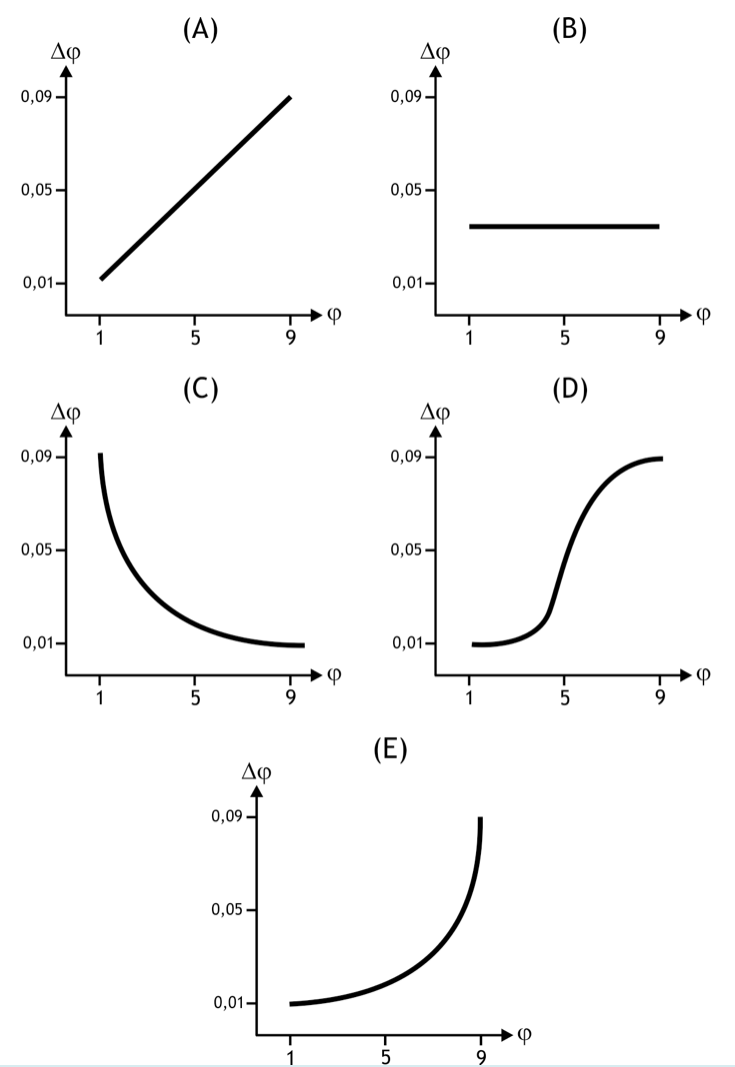
\includegraphics[width=\textwidth]{weber_IMPP.png}
\end{center}
\end{column}

\end{columns}
    
\end{frame}



\begin{frame}{IMPP Frage}


\begin{columns}[c]
\begin{column}{6cm}
Die Kenntnis der relativen Empfindlichkeit von Sinnessystemen spielt in der klinischen Diagnostik eine große Rolle. 

Welche der folgenden Abbildungen zeigt in diesem Zusammenhang am besten die Beziehung zwischen \textcolor{theme}{notwendigem Reizzuwachs} (\( \Delta \varphi \)) und \textcolor{theme}{Größe des Ausgangsreizes} (\(\varphi\)) für eine erfolgreiche Reizdiskriminiation? \\[0.2 cm]


\textcolor{theme}{Webersches Gesetz: \(\frac{\Delta \varphi}{\varphi}\) ist konstant!}


\end{column}


\begin{column}{5cm}
\begin{center}
    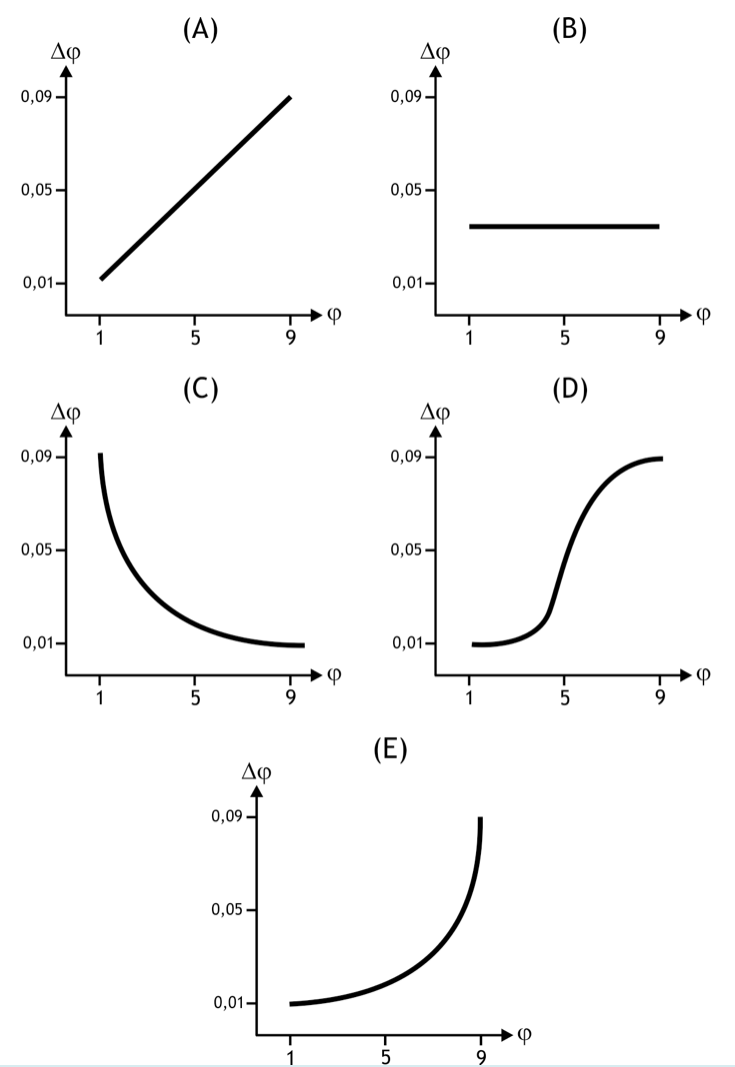
\includegraphics[width=\textwidth]{weber_IMPP.png}
\end{center}
\end{column}

\end{columns}
    
\end{frame}




%% %% %% %% Review



\begin{frame}

 \frametitle{Jetzt* sollten Sie folgendes können}



\begin{block}{Grundlagen:}




\begin{itemize}

    \item 
Die Begriffe Modalität, Qualität und Intensität erklären
    \item 
Erklären, was eine Schwellenbestimmung ist 
    \item 
Die Gesetze von Weber/Fechner und Stevens anführen und anwenden
    \item 
Adäquate Reize definieren
    \item 
Den allgemeinen Weg der Wahrnehmung vom Reiz zu den entsprechenden Zentren im Gehirn erläutern 
    \item 
Effekte von neuronalen Netzwerken auf die Reizwahrnehmung erklären
\end{itemize}


\end{block}



 

\begin{block}{Klinik:}

\begin{itemize}
    
\item 
Methoden zur Bestimmung von Schwellen erläutern 
\item
Agnosie erklären und ein Beispiel geben
\item
Synästhesie erklären und ein Beispiel geben


\end{itemize}


\end{block}



\end{frame}

\begin{frame}{Danke für Ihr Feedback}

\begin{center}
    
\includegraphics[width=0.5\textwidth]{feedback_QR.png}
\end{center}

\url{https://forms.office.com/e/hgdEawgrY5}

\end{frame}



%% %% %% Bildnachweis
\begin{frame}
\frametitle{Bildnachweis}
\begin{tiny}



 
\begin{itemize}


\item
Aktionspotential. Action\_potential.svg: Original by en:User:Chris 73, updated by en:User:Diberri, converted to SVG by tiZomderivative work: de:Benutzer:Jnns, CC BY-SA 3.0 \url{http://creativecommons.org/licenses/by-sa/3.0/}, via Wikimedia Commons

\item
Aktivierung von Haarzellen. Von Schneider00 - Eigenes Werk, CC BY-SA 3.0, \url{https://commons.wikimedia.org/w/index.php?curid=15974126}

\item
Apfel vor türkisem Hintergrund. Photo by \href{https://unsplash.com/@louishansel?utm_source=unsplash&utm_medium=referral&utm_content=creditCopyText}{Louis Hansel} on \href{https://unsplash.com/s/photos/apple?utm_source=unsplash&utm_medium=referral&utm_content=creditCopyText}{Unsplash}
  
\item
Ausgestreckte Hand mit Apfel. Photo by \href{https://unsplash.com/@priscilladupreez?utm_source=unsplash&utm_medium=referral&utm_content=creditCopyText}{Priscilla Du Preez} on \href{https://unsplash.com/s/photos/apple?utm_source=unsplash&utm_medium=referral&utm_content=creditCopyText}{Unsplash}
  
  

\item
Beispiele aus einem Test zur Unterscheidung von Farben. Screenshot aus der \href{https://melamela.shinyapps.io/colour_vision/}{Colour vision test app}, meine eigene Arbeit, CC-BY-SA 4.0, 2021. 

\item
Bunte Türen in einem mehrstöckigen Gebäude.Photo by \href{https://unsplash.com/@withluke?utm_source=unsplash&utm_medium=referral&utm_content=creditCopyText}{Luke Stackpoole} on \href{https://unsplash.com/s/photos/colours?utm_source=unsplash&utm_medium=referral&utm_content=creditCopyText}{Unsplash}
  
\item
Evelyn Glennie. Photo, may 30, 2004- photo: nomo/michael hoefner \url{http://www.zwo5.de} CC-BY-SA 2.5 via Wikimedia Commons.

\item 
Frau mit großem Einkaufskorb. Photo by \href{https://unsplash.com/@ibilyk?utm_source=unsplash&utm_medium=referral&utm_content=creditCopyText}{Liuba Bilyk} on \href{https://unsplash.com/s/photos/carrying-groceries?utm_source=unsplash&utm_medium=referral&utm_content=creditCopyText}{Unsplash}
  
  \item
  Geometrische Figuren unterschiedlicher Farbintensität zur Feststellung der Sehschwelle. Mein eigenes Werk, CC-BY-SA 4.0, 2022.
  
  \item
  G-protein gekoppelter Rezeptor vom Typ G\textsubscript{S}. Takanori Nakane, CC BY-SA 3.0 \url{https://creativecommons.org/licenses/by-sa/3.0}, via Wikimedia Commons
 
 \item
 Graphen zur Darstellung, wie sich das Gesetz von Weber und Fechner aus dem Weberschen Gesetz ableitet. Mein eigenes Werk, CC-BY-SA 4.0, 2022. 
 
\item
Handschuh. Photo by Vince Fleming on Unsplash. 
  \end{itemize}
\end{tiny}
\end{frame}



\begin{frame}
\frametitle{Bildnachweis}
\begin{tiny}



 
\begin{itemize}

\item 
Ankündigung Progress Test. Von Rainer Petzina, Medical School Hamburg, mit Erlaubnis.
  
  
\item
Illustration des Gesetzes von Weber und Fechner mit Punkten. By Д.Ильин: vectorization - File:Weber-Fechner law demo - dots.png by MrPomidor, CC0, \url{https://commons.wikimedia.org/w/index.php?curid=113926988}
  
\item
Ingenieurin schreibt mathematische Formeln an eine Tafel. Photo by \href{https://unsplash.com/@thisisengineering?utm_source=unsplash&utm_medium=referral&utm_content=creditCopyText}{ThisisEngineering RAEng} on \href{https://unsplash.com/s/photos/formula?utm_source=unsplash&utm_medium=referral&utm_content=creditCopyText}{Unsplash}
  

\item
Kiki und Bouba.  Monochrome version 1 June 2007 by BendžVectorized with Inkscape --Qef (talk) 21:21, 23 June 2008 (UTC), CC BY-SA 3.0 \url{http://creativecommons.org/licenses/by-sa/3.0/}, via Wikimedia Commons
  
  
\item
"Klassische" fünf Sinne. Jason Wirchin, CC0, via \href{ https://commons.wikimedia.org/wiki/File:Five_Senses.jpg}{Wikimedia Commons}

\item
Klaviatur mit Ton-Farbe-Zuordnung nach Skrjabin. JPEG by Ziga; PNG by Romanm; SVG by Connum. - original PNG page is/was here; SVG drawing: own work, Gemeinfrei, \url{https://commons.wikimedia.org/w/index.php?curid=4021885}


\item

Kontrastverschärfung durch laterale Hemmung. Von Zsynth, CC BY-SA 3.0, \url{https://commons.wikimedia.org/w/index.php?curid=1645056 }

\item
Luftballons mit frohen und traurigen Smileys. Photo by \href{https://unsplash.com/@artbyhybrid?utm_source=unsplash&utm_medium=referral&utm_content=creditCopyText}{Hybrid} on \href{https://unsplash.com/s/photos/feedback?utm_source=unsplash&utm_medium=referral&utm_content=creditCopyText}{Unsplash}


\item
Naive Sicht auf Wahrnehmungsprozesse. Mein eigenes Werk, CC-BY-SA 4.0, 2021.

\item 
Papier-Lose. Photo by \href{https://unsplash.com/@melpoole?utm_content=creditCopyText&utm_medium=referral&utm_source=unsplash}{Mel Poole} on \href{https://unsplash.com/photos/gT-Sob4njj8?utm_content=creditCopyText&utm_medium=referral&utm_source=unsplash}{Unsplash}
  

\item
Party. Photo by \href{https://unsplash.com/@johnarano?utm_source=unsplash&utm_medium=referral&utm_content=creditCopyText}{John Arano} on \href{https://unsplash.com/s/photos/party?utm_source=unsplash&utm_medium=referral&utm_content=creditCopyText}{Unsplash}
  
  \item
  Rhodopsin. By Roland Deschain - Palczewski K, et al ("Crystal structure of rhodopsin: A G protein-coupled receptor." Science. 2000 Aug 4;289(5480):739-45 NOTE: Originally uploaded 06:06, 25 June 2006 (UTC) (log) to en:wikipedia by Roland Deschain with the following summary: "This image was created by myself using the free public software "Western Barley Protein Workshop". The PDB file (Accession #1F88) was obtain from Research Collaboratory for Structural Bioinformatics Protein Data Bank (http://www.rcsb.org/pdb/Welcome.do). The protein was crystallized and published by Palczewski K, et al ("Crystal structure of rhodopsin: A G protein-coupled receptor." Science. 2000 Aug 4;289(5480):739-45.)". Public Domain
  
\item
Schmerzskala. Von Cvf-ps - Eigenes Werk, CC BY 3.0, \url{https://commons.wikimedia.org/w/index.php?curid=18315596}

\item
Stillleben mit Kaffee. Photo by \href{https://unsplash.com/@garrethpb?utm_source=unsplash&utm_medium=referral&utm_content=creditCopyText}{Garreth Paul} on \href{https://unsplash.com/s/photos/still-life?utm_source=unsplash&utm_medium=referral&utm_content=creditCopyText}{Unsplash}

\item
Synaesthesia: Painting by Numbers (2022). Felicity Inkpen, \url{felicityinkpen.co.uk}, \url{@felicityinkpen}, mit Erlaubnis der Künstlerin.

  
\item
(Theoretischer) Graph zur Bestimmung der Reizschwelle. Mein eigenes Werk, CC BY-SA 4.0, 2022.

\item
Wahrnehmungsbahn und einzelne Prozesse entlang der Wahrnehmungsbahn (mehrere Bilder). Mein eigenes Werk, CC BY-SA 4.0, 2022. 
  
  \item
Zwei Frauen im Gespräch vor einem Laptop. Photo by \href{https://unsplash.com/@mimithian?utm_source=unsplash&utm_medium=referral&utm_content=creditCopyText}{Mimi Thian} on \href{https://unsplash.com/s/photos/discussion?utm_source=unsplash&utm_medium=referral&utm_content=creditCopyText}{Unsplash}
  
  
\end{itemize}
\end{tiny}
\end{frame}






\end{document}

%%% Frequently used snippets

%% \begin{columns}[c]

%% \begin{column}{5cm}
%% \end{column}

%% \begin{column}{5cm}
%% \end{column}


%% \end{columns}




